\documentclass[a4paper]{article}
\usepackage[noend, noline, ruled]{algorithm2e}
\usepackage{tikz}
\usepackage{paralist,expdlist}
\usepackage[margin=1in]{geometry}
\usepackage{amsmath,amsthm}
\usepackage{amssymb}
\usepackage{authblk}
\usepackage{array}
\usepackage[utf8]{inputenc}
\usepackage[T1]{fontenc}
\usepackage{enumitem}
\usepackage{stmaryrd}
\usepackage{xcolor, colortbl}
\usepackage{thmtools}
\usepackage{mathtools}
\usepackage{thm-restate}
\usepackage{microtype}
\usepackage{lmodern}
\usetikzlibrary{snakes}


\usepackage{lineno}

\usepackage[colorlinks]{hyperref}
\usepackage[capitalise]{cleveref}

\crefname{subappendix}{Appendix}{Appendices}
\crefname{appendix}{Appendix}{Appendices}
\crefname{section}{Section}{Sections}
\crefname{figure}{Figure}{Figures}

\setenumerate{itemsep=0pt,topsep=2pt,parsep=0pt,partopsep=0pt}
\setitemize{itemsep=0pt,topsep=2pt,parsep=0pt,partopsep=0pt}


\usetikzlibrary{decorations.pathreplacing,decorations.pathmorphing}

\pagestyle{plain}

\newtheorem{theorem}{Theorem}[section]
\newtheorem{fact}[theorem]{Fact}
\newtheorem{lemma}[theorem]{Lemma}
\newtheorem{corollary}[theorem]{Corollary}
\newtheorem{proposition}[theorem]{Proposition}
\newtheorem{observation}[theorem]{Observation}

\theoremstyle{definition}
\newtheorem{definition}[theorem]{Definition}
\newtheorem{construction}[theorem]{Construction}

\newtheorem{claim}[theorem]{Claim}
\theoremstyle{remark}
\newtheorem{example}[theorem]{Example}
\newtheorem{remark}[theorem]{Remark}

\crefname{section}{Section}{Sections}
\crefname{construction}{Construction}{Constructions}
\crefname{claim}{Claim}{Claims}
\crefname{fact}{Fact}{Facts}


\usepackage{tikz-qtree}
\usetikzlibrary{decorations.pathreplacing,decorations.pathmorphing}
\usetikzlibrary{shapes,arrows}
\usetikzlibrary{shapes.multipart}
\usetikzlibrary{decorations.text}
\usetikzlibrary{calc}



\newcommand{\IPMFull}{\textsc{Internal Pattern Matching Queries}\xspace}
\newcommand{\IPM}{\textsc{IPM Queries}\xspace}
\newcommand{\IPMOne}{\textsc{IPM Query}\xspace}
\newcommand{\RIPM}{\textsc{Restricted IPM Queries}\xspace}
\newcommand{\RIPMOne}{\textsc{Restricted IPM Query}\xspace}
\newcommand{\PQ}{\textsc{Period Queries}\xspace}
\newcommand{\BQ}{\textsc{Prefix-Suffix Queries}\xspace}
\newcommand{\BQone}{\textsc{Prefix-Suffix Query}\xspace}
\newcommand{\PEQ}{\textsc{Periodic Extension Queries}\xspace}
\newcommand{\FC}{\textsc{Cyclic Equivalence Queries}\xspace}
\newcommand{\BLCPFull}{\textsc{Bounded Longest Common Prefix (LCP) Queries}\xspace}
\newcommand{\BLCP}{\textsc{Bounded LCP Queries}\xspace}
\newcommand{\ILCP}{\textsc{Interval Longest Common Prefix (LCP) Queries}\xspace}
\newcommand{\ILCPFull}{\textsc{Interval Longest Common Prefix (LCP) Queries}\xspace}
\newcommand{\LSC}{\textsc{LZ Substring Compression Queries}\xspace}
\newcommand{\GSC}{\textsc{Generalized LZ Substring Compression Queries}\xspace}
\newcommand{\LCEQFull}{\textsc{Longest Common Extension Queries}\xspace}
\newcommand{\LCEQ}{\textsc{LCE Queries}\xspace}
\newcommand{\LCE}{\operatorname{LCE}\xspace}
\newcommand{\LZ}{\operatorname{LZ}}
\newcommand{\Zz}{\mathbb{Z}_{\ge 0}}

\newcommand{\pillar}{\ensuremath{\mathtt{PILLAR}}\xspace}

\renewcommand{\Pr}{\mathbb{P}}
\newcommand{\BB}{\mathcal{B}}

\newcommand{\TM}{\mathsf{TM}}

\newcommand{\SPEC}{\mathsf{SpRuns}}




\newcommand{\R}{\mathsf{Samples}}
\newcommand{\N}{\mathsf{NHP}}
\newcommand{\HP}{\mathsf{HP}}
\newcommand{\Y}{\mathsf{Y}}
\newcommand{\B}{\mathbf{B}}



\newcommand{\ceil}[1]{\left\lceil #1 \right\rceil}
\newcommand{\floor}[1]{\left\lfloor #1 \right\rfloor}
\newcommand{\intr}[1]{\llbracket #1 \rrbracket}
\newcommand{\eps}{\varepsilon}
\newcommand{\sub}{\subseteq}
\newcommand{\integ}{\mathbb{Z}}
\newcommand{\nat}{\mathbb{N}}
\newcommand{\sm}{\setminus}



\newcommand{\lcs}{\operatorname{lcs}}
\newcommand{\lcp}{\operatorname{lcp}}
\newcommand{\lcpinf}[2]{\lcp({#1}^\infty, {#2})}
\newcommand{\dd}{\mathinner{\ldotp\ldotp}}
\DeclareMathOperator{\per}{per}
\newcommand{\val}{\mathsf{val}}
\newcommand{\aalph}{\mathit{alph}}



\newcommand{\pred}{\mathrm{pred}}
\newcommand{\suc}{\mathrm{succ}}
\newcommand{\rank}{\mathrm{rank}}
\newcommand{\select}{\mathrm{select}}



\newcommand{\first}{\mathsf{first}}
\newcommand{\osiemsiedem}{\left(\tfrac{8}{7}\right)}
\newcommand{\Occ}{\mathit{Occ}}
\newcommand{\A}{\mathcal{P}}
\newcommand{\esigma}{\bar{\Sigma}}



\newcommand{\Rot}{\mathsf{rot}}
\newcommand{\ROT}{\mathsf{Rot}}
\newcommand{\Eval}{\mathcal{E}}
\newcommand{\Exp}{\mathbb{E}}
\newcommand{\T}{\mathcal{T}_{\sf suf}}
\newcommand{\maybeqed}{}
\newcommand{\RUNS}{\mathsf{RUNS}}
\newcommand{\Runs}{\mathsf{R}}
\newcommand{\MaxReg}{\mathsf{MaxReg}}
\newcommand{\Mid}{\mathsf{Mid}}
\newcommand{\MidBlock}{\mathsf{MidBlock}}
\newcommand{\code}{\mathsf{code}}


\newcommand{\Oh}{\mathcal{O}}

\newcommand{\parent}{parent}
\newcommand{\rchild}{rchild}
\newcommand{\lchild}{lchild}
\renewcommand{\S}{\mathsf{Sync}}
\renewcommand{\S}{\mathsf{Sync}}
\newcommand{\F}{\mathsf{F}}
\newcommand{\SF}{\mathsf{SyncFr}}

\newcommand{\layer}[1]{\floor{\log(\frac23(#1+1))}}


\newcommand{\rsucc}{\mathit{rsucc}}

\newcommand{\BLOCK}{\mathsf{Block}}
\newcommand{\run}{\mathsf{run}}
\newcommand{\id}{\mathsf{id}}
\newcommand{\len}{\mathsf{len}}

\DeclareMathOperator{\argmin}{arg min}

\newcommand{\BF}{\mathit{F}}

\setlength{\fboxsep}{5pt}
\newsavebox{\mybox}
\newenvironment{dsproblem}[1]
{\begin{center}\begin{lrbox}{\mybox}\begin{minipage}{0.96\columnwidth}{\textsc{#1}}\\}
{\end{minipage}\end{lrbox}\fbox{\usebox{\mybox}}\end{center}}


  \newcommand{\defdsproblem}[2]{
  \begin{dsproblem}{#1}
#2
  \end{dsproblem}
  }





\title{Internal Pattern Matching Queries in~a Text and Applications\thanks{A preliminary version of this work was presented at the 26th Annual {ACM-SIAM} Symposium on Discrete Algorithms (SODA 2015)~\cite{DBLP:conf/soda/KociumakaRRW15} and included in the Ph.D.\ thesis of the first author~\cite{phd}.}}

\renewcommand\Affilfont{\normalsize}


\author[1]{Tomasz Kociumaka}
\author[2,3]{Jakub Radoszewski}
\author[2]{Wojciech Rytter}
\author[2]{Tomasz Wale\'n}
 
\affil[1]{Max Planck Institute for Informatics,  Saarbrücken, Germany}
\affil[ ]{\texttt{tomasz.kociumaka@mpi-inf.mpg.de}}
 \affil[2]{University of Warsaw, Warsaw, Poland}
 \affil[ ]{\texttt{[jrad, rytter, walen]@mimuw.edu.pl}}
 \affil[3]{Samsung R\&D Warsaw, Warsaw, Poland}

\date{\empty}


\begin{document}
\maketitle

\begin{abstract}
We consider several types of internal queries, that is, questions about \emph{fragments} of a given text 
specified in constant space by their locations in .
Our main result is an optimal data structure for Internal Pattern Matching (IPM) queries which,
given two fragments  and , ask for a representation of all fragments contained in  and matching  exactly.
This problem can be viewed as an internal version of the fundamental Exact Pattern Matching problem:
we are looking for occurrences of one substring of  within another substring.
Our data structure answers IPM queries in time proportional to the quotient  of fragments' lengths,
which is required due to the information content of the output.
If  is a text of length  over an integer alphabet of size ,
then our data structure occupies  machine words (that is,  bits)
and admits an -time construction algorithm.

We show the applicability of IPM queries for answering internal queries corresponding to other classic string processing problems.
Among others, we derive optimal data structures reporting the periods of a fragment and testing the cyclic equivalence of two fragments.
Since the publication of the conference version of this paper (SODA 2015), IPM queries
have found numerous further applications, following the path paved by the classic Longest Common Extension (LCE) queries of Landau and Vishkin (JCSS, 1988).
In particular, IPM queries have been implemented in grammar-compressed and dynamic settings
and, along with LCE queries, constitute elementary operations of the \pillar model, developed by Charalampopoulos, Kociumaka, and Wellnitz
(FOCS 2020) to design universal approximate pattern-matching algorithms.

All our algorithms are deterministic, whereas the data structure in the conference version of the paper only admits randomized construction in  expected time.
To achieve this, we provide a novel construction of \emph{string synchronizing sets} of Kempa and Kociumaka (STOC 2019).
Our method, based on a new \emph{restricted} version of the recompression technique of Jeż (\emph{J.\ ACM}, 2016),
yields a hierarchy of  string synchronizing sets covering the whole spectrum of fragments' lengths.
\end{abstract}


\section{Introduction}
In this paper, we consider \emph{internal queries}, which ask to solve instances of a certain string processing problem with input strings given as fragments of a fixed string  represented by their endpoints. The task is to preprocess , called the \emph{text}, into a data structure that efficiently answers certain types of internal queries.
In more practical applications, the text  can be interpreted as a corpus containing all the data gathered for a given study
(such as the concatenation of genomes to be compared).
On the other hand, when internal queries arise during the execution of algorithms, then  is typically the input to be processed.

The setting of internal queries does not include problems like text indexing, where the text is available in advance but the pattern is explicitly provided at query time.
This restricts the expressibility of internal queries but at the same time allows for greatly superior query times, which do not need to account for reading any strings.
Another difference is in the typical usage scenario: Data structures for indexing problems are primarily designed to be interactively queried by a user.
In other words, they are meant to be constructed relatively rarely, but they need to be stored for prolonged periods of time.
As a result, space usage (including the multiplicative constants) is heavily optimized, while the efficiency of construction procedures is of secondary importance.
On the other hand, internal queries often arise during bulk processing of textual data.
The relevant data structures are then built within the preprocessing phase of the enclosing algorithms, 
so the running times of the construction procedures are counted towards the overall processing time. 
In this setting, efficient construction is as significant as fast queries. 

The origins of internal queries in texts can be traced back to the invention of the \LCEQFull (\LCEQ),
originally introduced by Landau and Vishkin~\cite{DBLP:journals/jcss/LandauV88}.
In such a query, given two fragments of the text , one is to compute the length of their longest common prefix.
The classic data structure for \LCEQ takes linear space, supports constant-time queries, and can be constructed in linear time~\cite{DBLP:journals/siamcomp/HarelT84,DBLP:journals/jcss/LandauV88,DBLP:journals/jacm/Farach-ColtonFM00}.
Although this trade-off is optimal for large alphabets, a text of length  over an alphabet of size  can, in general, be stored in  bits (which is  machine words) and read in  time.
Only recently, Kempa and Kociumaka~\cite{phd,Kempa2019} showed that such complexity and preprocessing time are sufficient for constant-time \LCEQ. 

Components with optimal deterministic construction and constant-time queries are particularly valued,
because algorithms can use them essentially for free,
i.e., with no negative effect on the overall complexity in the standard theoretical setting.
We develop data structures with such guarantees for internal versions of several natural problems in text processing, including Exact Pattern Matching.

We always denote the input text by  and its length by .
We also make a standard assumption (cf.\ \cite{DBLP:journals/jacm/Farach-ColtonFM00}) that the characters of  are (or can be identified with) integers 
\footnote{ For , we
denote , , and . },
where the , that is,  is over a polynomially-bounded \emph{integer alphabet}.
Our results are designed for the standard word RAM model with machine words of  bits\footnote{Throughout this paper,  denotes the base-2 logarithm (any other base is explicitly provided in the subscript).}.
In this model, the text  can be represented using  machine words, that is,  bits, in a
so-called packed representation; see~\cite{DBLP:journals/tcs/Ben-KikiBBGGW14}.

Before we formally state our results, let us recall a few elementary notations related to strings;
a more thorough exposition is provided in \cref{chp:prelim}.
For an alphabet  and an integer , by  we denote the set of length- strings over .
For a string , by  we denote its length and by  its subsequent characters.
We call  a \emph{fragment} of ; it can be interpreted as a range  of positions in~.
The fragment is called a \emph{prefix} if  and a \emph{suffix} if .
A fragment  corresponds to a substring of , that is, a string composed of letters .
Let us note that many fragments can correspond to (be occurrences of) the same substring.
The \emph{concatenation} of two strings  is denoted  or~.
We identify strings of length 1 with the underlying characters, which lets us write .
The length of the longest common prefix of two strings  is denoted by .
For a string  and an integer , we denote the concatenation of  copies of  by .
An integer  is a \emph{period} of a string  if  and  for all .
The smallest period of  is denoted as .

\subsection{Internal Pattern Matching (IPM) Queries}
Our main contribution here is a data structure
for the internal version of the Exact Pattern Matching problem,
which asks for the occurrences of one fragment within another fragment.

\defdsproblem{\textsc{Internal Pattern Matching (IPM) Queries}}{Given fragments  and  of 
  satisfying , report the fragments matching  and contained in  (represented as an arithmetic progression of starting positions).}
Let us note that if , then one can  ask  \IPM 
(for the occurrences of  within fragments of length  contained in , with overlaps of at least  characters between the subsequent fragments) and output  arithmetic progressions.
We impose the restriction  so that the output can be represented in constant space using the following folklore fact:

\begin{fact}[Breslauer and Galil~\cite{DBLP:journals/algorithmica/BreslauerG95}, Plandowski and Rytter~\cite{DBLP:conf/icalp/PlandowskiR98}]\label{fct:single}
  Let ,  be strings satisfying .
  The set of starting positions of the occurrences of  in  forms a single arithmetic progression.
\end{fact}

We design an optimal data structure for \IPM.

\begin{restatable}[Main result]{theorem}{thmipm}\label{thm:ipm}
  For every text , there exists a data structure of size  which answers \IPM in  time.  The data structure can be constructed in  time given the packed representation of .
\end{restatable}

Linear-time solutions of the exact pattern matching problem~\cite{morris1970linear,DBLP:journals/siamcomp/KnuthMP77,DBLP:journals/cacm/BoyerM77} are among the foundational results of string algorithms.
Although this alone can motivate the study of \IPM, the significance of our result is primarily due to a growing collection of applications.
In this work, we show that several further internal queries can be answered efficiently using \cref{thm:ipm}; these are described in detail in \cref{subsec:app}.
Other applications of \IPM, developed after the conference version of the paper~\cite{DBLP:conf/soda/KociumakaRRW15}, are listed in~\cref{sec:alien}.

\subsection{Applications of IPM Queries}\label{subsec:app}
\paragraph{\underline{Period Queries}.}
One of the central notions of combinatorics on words is that of a \emph{period} of a string.
Already Knuth, Morris, and Pratt~\cite{morris1970linear,DBLP:journals/siamcomp/KnuthMP77}
provided a linear-time procedure listing all periods of a given string (as a side result of their linear-time pattern-matching algorithm).

The sorted sequence of periods of a length- string can be cut into  arithmetic progressions~\cite{DBLP:journals/siamcomp/KnuthMP77}.
A complete characterization of the possible families of periods~\cite{DBLP:journals/jct/GuibasO81} further shows
that the size of such a representation ( bits) is asymptotically tight.
Hence, we adopt it in the internal version of the problem of finding all periods of a string,
formally specified below.

\defdsproblem{\PQ}{Given a fragment  of , report all periods of  (represented by disjoint arithmetic progressions).}

We have introduced \PQ in~\cite{DBLP:conf/spire/KociumakaRRW12},
presenting two solutions. 
The first data structure takes  space and answers \PQ in the optimal  time
after -time randomized construction.
The other one is based on orthogonal range searching;
its size is  and the query time is ,
where  and 
are analogous values for data structures answering range successor queries; see~\cref{sec:GSC} for a definition.
The state-of-the-art trade-offs are  and  for every constant ~\cite{DBLP:conf/swat/NekrichN12},
 and ~\cite{DBLP:journals/ipl/Zhou16},
as well as  and  for every constant ~\cite{DBLP:journals/tcs/CrochemoreIKRTW12}.
The first two of these data structures can be constructed in time ~\cite{DBLP:conf/soda/BelazzouguiP16,Gao2020},
and the third one in time ~\cite{DBLP:journals/tcs/CrochemoreIKRTW12}.

In this paper, we develop an asymptotically optimal data structure answering \PQ.

\begin{restatable}{theorem}{thmapppq}\label{thm:app-pq}
For every text , there exists a data structure of size  which answers \PQ in  time.
The data structure can be constructed in  time given the packed representation of .
\end{restatable}

Our query algorithm is based on the intrinsic relation between periods and \emph{borders} (i.e., substrings being both prefixes and suffixes) of a string.
In fact, to answer each \textsc{Period Query}, it combines the results of the following \BQ
used with  to determine the borders of~.

\defdsproblem{\BQ}{Given fragments  and  of  and a positive integer , report all suffixes of  of length in 
that also occur as prefixes of  (represented as an arithmetic progression of their lengths).}

In other words, we prove the following auxiliary result.

\begin{restatable}{theorem}{thmappbq}\label{thm:app-bq}
For every text , there exists a data structure of size  which answers \BQ in  time. The data structure can be constructed in  time given the packed representation of .
\end{restatable}

In many scenarios, very long periods ( for a string of length ) are irrelevant.
The remaining periods correspond to borders of length  and thus can be retrieved with just a constant number of \BQ.
The case of  is especially important
since fragments  with periods not exceeding , called \emph{periodic} fragments, can be uniquely extended to \emph{maximal repetitions}, also known as \emph{runs} (see~\cref{chp:prelim}).
We denote the unique run extending a periodic fragment  by .
If  is not periodic, we leave  undefined, which we denote as .

\defdsproblem{\PEQ}{Given a fragment  of , compute the run  extending .}

\noindent
\cref{thm:app-bq}, along with the optimal data structure for \LCEQ~\cite{Kempa2019}, imply the following result.

\begin{restatable}{theorem}{thmrun}\label{thm:run}
  For every text , there exists a data structure of size  which answers \PEQ in  time. The data structure can be constructed in  time given the packed representation of .
\end{restatable}

Bannai et al.~\cite{DBLP:journals/siamcomp/BannaiIINTT17} presented an alternative implementation of \PEQ with -time construction and -time queries.
The underlying special case of \PQ also generalizes \textsc{Primitivity Queries}
(asking if a fragment  is \emph{primitive}, i.e., whether it does not match  for any string  and integer ),
earlier considered by Crochemore et al.~\cite{DBLP:journals/tcs/CrochemoreIKRRW14},
who developed a data structure of size  with  -time query algorithm.

\paragraph{\underline{Cyclic Equivalence Queries}.}
We consider a \emph{rotation} operation which moves the last character of a given string  to the front.
Formally, if , then .
In general, for , we define the  function as the th function power of .
Two strings  and  are called cyclically equivalent if  for some integer .
A classic linear-time algorithm for checking cyclic equivalence of strings  and  consists in pattern matching for  in ~\cite{DBLP:journals/ipl/Manacher76}; there is also a simple linear-time constant-space algorithm~\cite{Jewels}.
We consider the following queries.

\defdsproblem{\FC}{
Given two fragments  and  of , return  (represented as an arithmetic progression).
}

\begin{restatable}{theorem}{thmfc}\label{thm:app-fc}
  For every text , there exists a data structure of size  which answers \FC in  time. The data structure can be constructed in  time given the packed representation of .
\end{restatable}

\paragraph{\underline{Bounded LCP Queries}.}
Keller et al.~\cite{DBLP:journals/tcs/KellerKFL14} used the following queries in the solution to their \GSC problem:
\defdsproblem{\BLCPFull}{Given two fragments  and  of , find the longest prefix  of  which  occurs in .}

Our result for \IPM can be combined with the techniques of~\cite{DBLP:journals/tcs/KellerKFL14} in a more efficient implementation of \BLCP.
Compared to the original version, the resulting data structure,
specified below, has a  factor instead of a  factor in the query time.

\begin{restatable}{theorem}{thmblcp}\label{thm:blcp}
For every text  of length  over an alphabet , there exists a data structure of size 
which answers \BLCP in  time.
The data structure can be constructed in  time.
\end{restatable}

In \cref{chp:app}, we formally define \GSC and discuss how \cref{thm:blcp} lets us improve and extend the results of~\cite{DBLP:journals/tcs/KellerKFL14}.

\paragraph{\underline{Earlier Versions of Our Results}.}
Weaker versions of \cref{thm:ipm,thm:app-pq,thm:app-bq,thm:run,thm:app-fc} (with  space and construction time) and \cref{thm:blcp} were published in the conference version of the paper~\cite{DBLP:conf/soda/KociumakaRRW15} and the Ph.D.\ thesis of the first author~\cite{phd}. Moreover, the construction algorithms provided in~\cite{DBLP:conf/soda/KociumakaRRW15} were Las-Vegas randomized, with linear bounds on the \emph{expected} running time only.

\subsection{Further Applications of IPM Queries}\label{sec:alien}
Since the publication of the conference version of this work~\cite{DBLP:conf/soda/KociumakaRRW15}, 
the list of internal queries, predominantly implemented using \IPM, has grown to include
shortest unique substrings~\cite{DBLP:journals/algorithms/Abedin0PT20},
longest common substring~\cite{DBLP:journals/corr/abs-1804-08731},
suffix rank and selection~\cite{WaveletSuffixTree,DBLP:conf/cpm/Kociumaka16},
BWT substring compression~\cite{WaveletSuffixTree},
shortest absent string~\cite{DBLP:journals/tcs/BadkobehCKP22},
dictionary matching~\cite{DBLP:journals/algorithmica/Charalampopoulos21},
string covers~\cite{DBLP:conf/spire/CrochemoreIRRSW20},
masked prefix sums~\cite{DBLP:conf/spire/Das0KMW22},
circular pattern matching~\cite{CPM2023}, and
longest palindrome~\cite{DBLP:conf/walcom/MitaniMSH23}.

Furthermore, \IPM have been used in efficient algorithms for many problems such
as approximate pattern matching~\cite{DBLP:conf/focs/Charalampopoulos20,DBLP:conf/focs/Charalampopoulos22},
approximate circular pattern matching~\cite{DBLP:journals/jcss/Charalampopoulos21,DBLP:conf/esa/Charalampopoulos22},
RNA folding~\cite{DBLP:conf/icalp/0001KS22},
and computing string covers~\cite{DBLP:conf/esa/RadoszewskiS20}.
Additionally, \IPM have found further indirect applications that are based on the internal queries from \cref{subsec:app}:
\PEQ have been applied for
approximate period recovery~\cite{DBLP:journals/tcs/AmirALS18,DBLP:journals/algorithmica/AmirBKLS22},
dynamic repetition detection~\cite{DBLP:conf/esa/AmirBCK19},
identifying two-dimensional maximal repetitions~\cite{DBLP:conf/esa/AmirLMS18},
enumeration of distinct substrings~\cite{DBLP:conf/spire/Charalampopoulos20},
and pattern matching with variables~\cite{DBLP:journals/toct/FernauMMS20,DBLP:conf/spire/KosolobovMN17},
whereas
\BQ have been applied for detecting gapped repeats and subrepetitions~\cite{DBLP:journals/jda/KolpakovPPK17,DBLP:journals/mst/GawrychowskiIIK18},
in the dynamic longest common substring problem~\cite{DBLP:journals/corr/abs-1804-08731},
and for computing the longest unbordered substring~\cite{DBLP:journals/corr/abs-1805-09924}.

The fundamental role of \IPM as a building block for the design of string algorithms
motivated their efficient implementation in the compressed and dynamic settings~\cite{DBLP:conf/focs/Charalampopoulos20}.
In particular, the \pillar model, introduced in~\cite{DBLP:conf/focs/Charalampopoulos20}
with the aim of unifying approximate pattern-matching algorithms across different settings, includes \IPM as one of the primitives.
It also includes \LCEQ, defined as , and \LCEQ on reversed strings,
as well as the following basic primitives:
\begin{itemize}
  \item : Given a string  and integers , retrieve the string .
  \item : Given a string  and a position , retrieve the character .
  \item : Retrieve the length  of the string .
\end{itemize}
The argument strings of \pillar primitives are represented as fragments of one or more strings in a given text collection .

Using an earlier version of \cref{thm:ipm}, providing -time deterministic construction~\cite{phd}, it has been observed \cite[Theorem 7.2]{DBLP:conf/focs/Charalampopoulos20} that, after -time preprocessing of a collection  of strings of total length ,
each \pillar operation can be performed in  time.
We improve upon this result using \cref{thm:ipm} to implement \IPM and
the following implementation of \LCEQ.
\begin{proposition}[Kempa and Kociumaka~\cite{Kempa2019}]\label{prop:lce}
For every text  of length  over alphabet , there exists a data structure of size  which answers \LCEQ in  time. The data structure can be constructed in  time given the packed representation of .
\end{proposition}

We apply elementary bit-wise operations for  queries
(the  and  queries are straightforward since  is represented by a pointer to  and the two endpoints  and ).
This gives the following result.

\begin{theorem}\label{thm:pillar}
A collection  of strings of total length  over alphabet 
can be preprocessed in  time so that each \pillar operation can be performed in  time.
\end{theorem}

Since the approximate pattern-matching algorithms of \cite{DBLP:conf/focs/Charalampopoulos20,DBLP:conf/focs/Charalampopoulos22,DBLP:conf/esa/Charalampopoulos22} are implemented in the \pillar model,
\cref{thm:pillar} immediately improves the running times for strings over small alphabets.
In particular, given a pattern , a text , and a threshold , the occurrences of  in  with at most  mismatches (substitutions) can be reported in time ,
whereas the occurrences with at most  edits (insertions, deletions, and substitutions) can be reported in time . In both cases, the improvement is that the  term, dominating the complexity of previous state-of-the-art solutions~\cite{DBLP:conf/stoc/ChanGKKP20,DBLP:conf/focs/Charalampopoulos22} for small values of , is replaced by . 
A similar phenomenon applies to circular pattern matching with at most  mismatches~\cite{DBLP:conf/esa/Charalampopoulos22}, where we achieve  time for the reporting version of the problem and  for the decision version.

\subsection{Related Queries}\label{sec:related}
Internal queries are not the only problems in the literature involving fragments of a static text.
Other variants include
Interval LCP queries~\cite{DBLP:conf/soda/CormodeM05,DBLP:journals/tcs/KellerKFL14},
Range LCP queries~\cite{DBLP:conf/cocoon/Abedin0HNSST18,RangeLCP,DBLP:conf/spire/AmirLT15,DBLP:conf/spire/PatilST13},
Substring Hashing queries~\cite{DBLP:conf/cpm/FarachM96,DBLP:conf/esa/Gawrychowski11,DBLP:conf/esa/GawrychowskiLN14},
fragmented Pattern Matching queries~\cite{DBLP:journals/talg/AmirLLS07,DBLP:conf/esa/GawrychowskiLN14},
and Cross-Document Pattern Matching queries~\cite{DBLP:journals/jda/KopelowitzKNS14}, to mention a few.
In particular, Interval LCP queries can be used to solve the decision version of \IPM.
Keller et al.~\cite{DBLP:journals/tcs/KellerKFL14}
showed how to answer the decision version of \IPM in  time
using a data structure of size  that can be constructed in  time.
The aforementioned query time is valid for arbitrary lengths  and ,
so the efficiency of this data structure is incomparable to our~\cref{thm:ipm}.

\subsection{Technical Contributions}\label{sec:techniques}
Below, we briefly introduce the most important technical contributions of our work.
We start with a high-level overview of our \IPM data structure for large alphabets,
that is, .
In this setting, the space and construction time bounds of \cref{thm:ipm} simplify to .

\paragraph{String Matching by Deterministic Sampling}\label{sec:samp}
The idea of (deterministic) sampling is a classic technique originally developed for parallel string matching algorithms~\cite{DBLP:journals/siamcomp/Vishkin91} and later applied in other contexts such as quantum string matching~\cite{DBLP:journals/jda/HariharanV03}.
Algorithms using this approach to find the occurrences of a pattern  in a text  follow a three-phase scheme.
In the preprocessing phase, a subset of characters of , called the \emph{sample}, is determined.
Then, in the filtering phase, the algorithm selects all fragments  of  that match the sample.
Finally, in the verification phase, the algorithm checks whether each candidate  matches the whole pattern .
The efficiency of this scheme hinges on two properties of the chosen samples: (1) they must be simple enough to support efficient filtering,
and (2) they must carry enough information to leave few candidates for the verification phase.
For example, Vishkin~\cite{DBLP:journals/siamcomp/Vishkin91} chooses a sample of size  so that the starting positions of the candidates surviving the filtering phase form  arithmetic progressions whose difference is the smallest period of~.

Our data structure answering \IPM, described in \cref{chp:ipm}, uses contiguous samples, that is, the sample of a pattern  can be interpreted as a fragment of  contained in . Moreover, we minimize the total number of samples across all the fragments of  rather than the size of each sample,
and we aim to choose the samples \emph{consistently}, so that any fragment matching a sample is a sample itself.
These constraints are infeasible for highly periodic () patterns, whose length is much larger than the smallest period (we set  as the cut-off point for the period), and such patterns are handled in \cref{chp:per} using different techniques outlined later on.
As for non-highly-periodic () patterns, we choose  samples in total so that the smallest period of the sample of  is .
The small number of samples allows storing them explicitly, whereas the large period guarantees that the sample of  has  occurrences within any fragment  of length  (due to \cref{fct:single}).
Thus, at query time, our data structure uses the precomputed set of samples (stored in appropriate deterministic dictionaries~\cite{DBLP:conf/icalp/Ruzic08,DBLP:conf/focs/PatrascuT14}) to identify the sample of  and its occurrences in .
Then, we use \LCEQ to test which of these occurrences extend to occurrences of~.

\paragraph{Sample Selection: String Synchronizing Sets Hierarchy and Restricted Recompression}
The challenge of implementing the strategy outlined above is to consistently pick  samples among  fragments of .
The natural first step is to restrict the selection to  fragments whose lengths form a geometric series,
but any further reduction in the number of samples requires non-trivial symmetry breaking.

In the conference version of this paper~\cite{DBLP:conf/soda/KociumakaRRW15}, we employed a strategy reminiscent of the \emph{minimizers} technique popular in bioinformatics~\cite{DBLP:journals/bioinformatics/RobertsHHMY04,Wood_2014,DBLP:journals/bioinformatics/DeorowiczKGD15,DBLP:journals/bioinformatics/Li18}
and known under different names in many other applications~\cite{DBLP:conf/sigmod/SchleimerWA03,DBLP:conf/icdm/SorokinaGWG06,DBLP:journals/ce/ButakovS09,DBLP:journals/tissec/PonecGWB10}.
In that approach, candidate fragments are consistently assigned uniformly random weights, and the sample of  is defined as the minimum-weight fragment of a certain length (such as ) contained in . 
With minor adaptations (necessary to avoid highly periodic samples), this scheme yields  length- samples in expectation for every .
Subsequently, our sample selection algorithm was adapted for answering \LCEQ~\cite{DBLP:conf/soda/BirenzwigeGP20,phd} and for the Burrows--Wheeler transform construction~\cite{Kempa2019}. The latter paper contributed the following clean notion, which has since been applied in many further contexts (see e.g.~\cite{DBLP:conf/focs/KempaK20,DBLP:conf/esa/Charalampopoulos21,DBLP:conf/stoc/KempaK22,DBLP:conf/soda/JinN23}).

\begin{restatable}[\textbf{Synchronizing Set}; Kempa and Kociumaka~\cite{Kempa2019}]{definition}{defsss}\label{def:sss}
  Let  be a string of length  and let .
  A set  is a
  \emph{-synchronizing set} of  if it satisfies the following conditions:
  \begin{description}
\item[Consistency:] For all , if  and the fragments  and  match, then .
\item[Density:]
For every , we have .
\end{description}
We say that the elements of a fixed -synchronizing set  are -\emph{synchronizing positions} and the fragments  for  are -\emph{synchronizing fragments}; the set of -synchronizing fragments is denoted~.
\end{restatable}

Kempa and Kociumaka~\cite{Kempa2019} obtained the following result building upon our original sample-selection algorithm~\cite{DBLP:conf/soda/KociumakaRRW15}
and its derandomized version presented in~\cite{phd}.
\begin{restatable}[{\cite[Proposition 8.10 and Theorem 8.11]{Kempa2019}}]{proposition}{prpsynch}\label{prp:synch}
For every text  with  and , there exists a -synchronizing set of size  that can be constructed in  time. Moreover, if  and  is given in a packed representation, then the construction time can be improved to .
\end{restatable}
It is not hard to argue (see \cref{lem:repr}) that one can pick as samples all the length- fragments as 
well as all the -synchronizing fragments for all  and some fixed -synchronizing sets.
Unfortunately, it takes  time to construct these synchronizing sets using the algorithm of \cref{prp:synch}.
Consequently, the deterministic version of \cref{thm:ipm} published in~\cite{phd} follows a sophisticated approach relying on just two string synchronizing sets, constructed in  time each.
In this paper, we apply a more natural strategy and show that the entire hierarchy of  -synchronizing sets
can be constructed in deterministic  time. Formally, our new result reads as follows:

\begin{restatable}[\bf Construction of Synchronizing Sets Hierarchy]{theorem}{thmsss}\label{thm:sss}
  After -time preprocessing of a text  with ,
  given , one can construct
  in  time a -synchronizing set  of size  .
  Moreover, no -synchronizing fragment induced by  has period .
\end{restatable}

As opposed to~\cite{Kempa2019}, our construction does not use minimizers, but we rely on 
locally consistent parsing, a concept dating back to mid-1990s~\cite{FirstConsistentParsing,SymmetryBreakingST,DBLP:conf/focs/SahinalpV96,DBLP:journals/algorithmica/MehlhornSU97}. Specifically, we adapt the \emph{recompression} technique of Jeż~\cite{DBLP:journals/talg/Jez15,DBLP:journals/jacm/Jez16},
which results in a simple and efficient parsing scheme.

All locally consistent parsing algorithms construct a sequence of factorizations of , where
level- phrases consist of single letters of , the only level- phrase (for some ) consists of the entire text ,
and, for each , the level- phrases are concatenations of level- phrases.
In this context, local consistency means that whether or not two subsequent level- phrases are grouped into the same level- phrase 
is a local decision that depends only on a few neighboring  level- phrases.
Unfortunately, the lengths of level- phrases can vary significantly between regions of the text, and thus it is not possible to make sure that the symmetry-breaking decisions are made based on fixed-size contexts, as required by the consistency property of string synchronizing sets (\cref{def:sss}).

Consequently, we alter the original recompression algorithm and introduce a small but consequential restriction: phrases that are deemed too long for their level are never merged with their neighbors. Although this trick does not eliminate very long phrases, it lets us quantify local consistency in terms of fixed-size contexts. In the following lemma, proved in \cref{sec:recompression}, the parameter  can be interpreted as the level- context size.
\begin{restatable}{lemma}{lemcons}\label{lem:cons}
Let  denote the set of starting positions of level- phrases (except for the leftmost one). 
Then, for every , if  and the fragments  and  match, then .
\end{restatable}

Restricted recompression has already been used in~\cite{DBLP:journals/tit/KociumakaNP23} to prove that every text admits a run-length straight-line program of a particular size.
Restricted variants of other locally consistent parsing schemes have been used in~\cite{DBLP:conf/latin/KociumakaNO22} and \cite{DBLP:conf/stoc/KempaK22} to derive efficient compressed and dynamic text indexes. In both cases, the counterpart of \cref{lem:cons} is what differentiates restricted variants from the original implementations of the locally consistent parsing schemes.

In \cref{chp:lce}, we provide further intuition and explain how to define the synchronizing sets in terms of the sets  of phrase boundaries.
\cref{sec:recompression} provides the formal definition and analysis of the restricted recompression technique.
The proof of \cref{thm:sss} is given in \cref{sec:correctness}.

\paragraph{\IPM in Highly Periodic Patterns}
As mentioned above, our deterministic sampling strategy applies only to non-highly-periodic () patterns.
In \cref{chp:per}, we develop a complementary data structure that is responsible for handling highly-periodic () patterns.

For this, we build upon the fact that the structure of highly-periodic fragments can be encoded by \emph{maximal repetitions} (also known as runs)~\cite{DBLP:journals/dam/Main89,DBLP:conf/focs/KolpakovK99,DBLP:journals/siamcomp/BannaiIINTT17}.
In particular, we rely on the notion of \emph{compatibility}~\cite{DBLP:journals/tcs/CrochemoreIKRRW14}: two strings are compatible whenever their 
string periods are cyclically equivalent.
If  is periodic, every matching fragment  can be extended to a run compatible with .
Moreover, due to the assumption , if  is contained within , then the run must contain the middle position of~.
Consequently, we develop a simple new data structure that, for any position in , in  time  
lists all runs with a certain minimum length (such as ) and maximum period (such as ). 
Next, we use the techniques of~\cite{DBLP:journals/tcs/CrochemoreIKRRW14} to eliminate runs incompatible with  
and find the occurrences of  within each compatible run.

\paragraph{\IPM in Texts over Small Alphabets}
The aforementioned techniques allow answering \IPM using  space and  construction time.
In the case of small alphabets, that is, , both complexities can be improved to .
For this, in \cref{sec:packed}, we reduce \IPM in  to \IPM in a text  of length 
over an alphabet of size . 
We use a -synchronizing set , constructed using \cref{prp:synch} for appropriate ,
to partition  into blocks, and we encode these blocks in .
By the density property of , each block has length at most  or shortest period at most .
Moreover, the consistency property implies that the block boundaries within  match the block boundaries within any occurrence of .
Consequently, we retrieve the fragments  and  of , encoding the blocks contained within  and , respectively,
identify the occurrences of  in , and apply \LCEQ (\cref{prop:lce}) through \cref{lem:peralg} below to check which of them correspond to occurrences of  in .
A major challenge in implementing this strategy is that  can be much longer than  despite .
In particular,  can be empty if  (in that case, we precompute the answers) or if  (in that case, we reuse the techniques for  patterns). In the remaining cases, we show that it suffices to trim  to a carefully defined fragment of length .

\paragraph{Applications of \IPM}
\cref{chp:app} demonstrates the usage of \IPM for answering \BQ, \FC, and \BLCP; it also covers applications of all these queries.
The common feature of our solutions is that we make a constant number of \IPM to list candidates (suffixes for \BQ, rotations for \FC, and previous occurrences for \BLCP), and then verify each of them using \LCEQ.
In the non-periodic case, verifying  candidates does not constitute any significant challenge. 
Otherwise, we exploit the structural insight of \cref{fct:single}: the sequence 
of reported starting positions forms a \emph{periodic progression}, meaning that ,
and thus, for any position , the answers to queries  can be obtained in bulk using just   queries. 
Formally, our main auxiliary result reads as follows:

\begin{restatable}{lemma}{peralg}\label{lem:peralg}
  Consider a text  equipped with a data structure answering \LCEQ in  time.
  Given a fragment  of  and a collection of fragments  represented with a periodic progression  and a position ,
  the following queries can be answered in  time:
  \begin{enumerate}[label=(\alph*)]
    \item\label{it:perpref} Report indices  such that  matches a prefix of , represented as a subinterval of .
     \item\label{it:permax} Report indices  maximizing , represented as a subinterval of .
  \end{enumerate}
\end{restatable}



\section{Strings and Periodicity}\label{chp:prelim}

We consider \emph{strings} over an \emph{alphabet} , i.e., finite sequences of \emph{characters} from the set~.
The set of all strings over  is denoted by , and  is the set of non-empty strings over .
Occasionally, we also work with the family  of \emph{infinite strings} indexed by non-negative integers.


\subsection{Basic Notations on Strings}\label{sec:comb}
Let us recall that, for a string , by  we denote its length, and by  its subsequent characters.
By  we denote the empty string.
By  we denote the set .
The string  is called the \emph{reverse} of .
A string  is called a \emph{substring} of  if 
for some  with .
In this case, we say that  \emph{occurs} in  at position~, and we denote by 
the \emph{occurrence} of  at position .
By  we denote the set of starting positions of all occurrences of  in .

We call  a \emph{fragment} of ; formally, a fragment can be interpreted as a tuple
consisting of (a pointer to) the string  and the two endpoints  with .
If a fragment  is an occurrence of a string , then we write  and say that  \emph{matches} .
Similarly, if  and  are occurrences of the same string, we denote this by ,
and we say that these fragments match.
On the other hand, the equality of fragments  is reserved for occasions when  is the same fragment as  (i.e.,  and ). 

We assume that a fragment  of a string  inherits some notions from the underlying substring: the \emph{length} , the characters  for , and the \emph{subfragments}  for  with .
A fragment  also has a natural interpretation as a \emph{range}  of positions in~.
This lets us consider \emph{disjoint} or \emph{intersecting} (\emph{overlapping}) fragments and define the containment relation () on fragments of . 
Moreover, for  with , the fragments  and  are called \emph{consecutive} and  is assumed to be their \emph{concatenation}.
If fragments  and  intersect, we denote their \emph{intersection}  by .
 
A fragment  of  of length  is called a \emph{proper} fragment of .
A fragment  is a \emph{prefix} of  if  and a \emph{suffix} of  if .
We extend the notions of a prefix and a suffix to the underlying substrings.  


We denote by  the natural order on 
and extend this order in the standard way to the \emph{lexicographic} order on .

The notion of concatenation  extends to  and , resulting in .
Also, the notion of the longest common prefix of two strings naturally extends to .
For a string , we also introduce the infinite power , i.e., the concatenation of infinitely many copies of .

\subsection{Periodic Structures in Strings}\label{sec:per_struct}
An integer  is a \emph{period} of a string  if  holds for all .
We call  \emph{periodic} if its smallest period satisfies .
A \emph{border} of a string  is a substring of  which occurs both as a prefix and as a suffix of~.
Note that  is a period of  if and only if  has a border of length .
Periods of a string  satisfy the following periodicity lemma.
\begin{lemma}[Periodicity Lemma~\cite{MR0162838,fine1965uniqueness}]\label{lem:per}
Let  be a string with periods  and .
If , then  is also a period of .
\end{lemma}

For an integer , the string  is called a \emph{power} of  (with \emph{root} ).
A string  is \emph{primitive} if it is not a power,
i.e.,  for every integer  and every root~.
For a string , the shortest string  that satisfies  for some  is called the \emph{primitive root} of .
Primitive strings enjoy a synchronizing property, which is an easy consequence of \cref{lem:per}.

\begin{lemma}[{see~\cite[{Lemma~1.11}]{AlgorithmsOnStrings}}]\label{lem:synchr}
A non-empty string  is primitive if and only if it occurs exactly twice in  (as a prefix and as a suffix).
\end{lemma}

By \cref{lem:synchr}, a string  is primitive if and only if it has exactly  distinct rotations.


\paragraph{Maximal Repetitions (Runs)}\label{sec:runs}
A \emph{run} (maximal repetition)~\cite{DBLP:journals/dam/Main89,DBLP:conf/focs/KolpakovK99} in a string  is a periodic fragment
 which can be extended neither to the left nor to the right without increasing the smallest period ,
that is,  and  provided that the respective positions exist.
We assume that runs are stored together with their periods so that  can be retrieved in constant time.
We denote the set of all runs in a string  by .


\begin{figure}[htpb]
\begin{center}
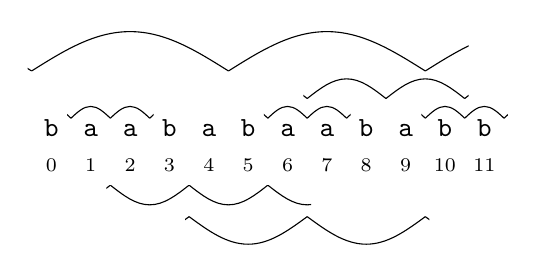
\begin{tikzpicture}[xscale=0.5,yscale=0.5]

\foreach \i/\x in {0/b,1/a,2/a,3/b,4/a,
                   5/b,6/a,7/a,8/b,9/a,
                   10/b,11/b}{
  \draw (\i,0) node[above] {\texttt{\x}};
  \draw (\i,-0.5) node {\scriptsize \i};
}

\foreach \ud in {0,5,9}{
  \begin{scope}[xshift=\ud cm,yshift=0.2cm]
  \clip (0.4,0.5) rectangle (2.6,1);
  \foreach \dx in {-1,0,1,2}{
    \draw[xshift=\dx cm] (0.5, 0.5) sin (1, 0.8) cos (1.5, 0.5);
  }
  \end{scope}
}

\begin{scope}
  \clip (6.4,1.1) rectangle (10.6,1.8);
  \foreach \dx in {-2,0,2,4}{
    \draw[xshift=\dx cm] (6.5, 1.2) sin (7.5, 1.7) cos (8.5, 1.2);
  }
\end{scope}

\begin{scope}[yshift=0.4cm]
  \clip (-0.6,1.4) rectangle (10.6,2.6);
  \foreach \dx in {-5,0,5,10}{
    \draw[xshift=\dx cm] (-0.5, 1.5) sin (2, 2.5) cos (4.5, 1.5);
  }
\end{scope}

\begin{scope}
  \clip (1.4,-1.7) rectangle (6.6,-1);
  \foreach \dx in {-2,0,2,4}{
    \draw[xshift=\dx cm] (1.5, -1) sin (2.5, -1.5) cos (3.5, -1);
  }
\end{scope}

\begin{scope}
  \clip (3.4,-2.6) rectangle (9.6,-1.8);
  \foreach \dx in {-3,0,3,6}{
    \draw[xshift=\dx cm] (3.5, -1.8) sin (5, -2.5) cos (6.5, -1.8);
  }
\end{scope}


\end{tikzpicture}
\end{center}
 \vspace*{-0.7cm}
\caption{\label{fig:run}
  Runs in .
}
\end{figure}

\begin{example}
  For a string , we have 
  see \cref{fig:run}.
  We have three runs with period 1:
  , , and ;
  two runs with period 2:  and ;
  one run with period 3: ;
  and one run with period 5: .
\end{example}

Our results rely on the following asymptotic bounds related to runs.

\begin{proposition}[\cite{DBLP:conf/focs/KolpakovK99,DBLP:journals/siamcomp/BannaiIINTT17}]\label{fct:runs}
Given a text  of length , the set  of all runs in  (together with their periods) can be computed in  time. In particular, .
\end{proposition}

\begin{figure}[th]
\begin{center}
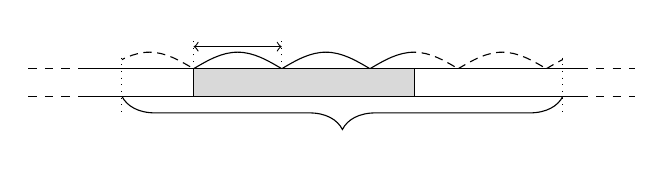
\begin{tikzpicture}[scale=0.7]

\filldraw[fill=black!15] (3,0) rectangle (7,.5);
\draw (1, 0) -- (10, 0);
\draw (1, .5) -- (10, .5);
\draw[dashed] (0,0) -- (1,0);
\draw[dashed] (0,.5) -- (1,.5);
\draw[dashed] (10,0) -- (11,0);
\draw[dashed] (10,.5) -- (11,.5);

\begin{scope}
\clip(3, 0.5) rectangle (7, 00.85);
\foreach \x in {3, 4.6, 6.2} {
	\draw (\x, 0.5) sin (\x+.8, .8) cos (\x + 1.6, 0.5);
}
\end{scope}

\begin{scope}
\clip(1.7, 0.5) rectangle (3, 00.85);
\foreach \x in {1.4} {
	\draw[densely dashed] (\x, 0.5) sin (\x+.8, .8) cos (\x + 1.6, 0.5);
}
\end{scope}
\begin{scope}
\clip(7, 0.5) rectangle (9.7, 0.85);
\foreach \x in {6.2, 7.8, 9.4} {
	\draw[densely dashed] (\x, 0.5) sin (\x+.8, .8) cos (\x + 1.6, 0.5);
}
\end{scope}

\draw (5, 0.25) node {};

\draw[dotted] (1.7, .7) -- (1.7, -.3);
\draw[dotted] (9.7, .7) -- (9.7, -.3);
\draw [decorate,decoration={brace,amplitude=12pt}] (9.7, 0) -- node[below=11pt] {} (1.7, 0);
\draw[dotted] (3, .5) -- (3,1);
\draw[dotted] (4.6, .5) -- (4.6, 1);
\draw[<->] (4.6, .9) -- node[above] {} (3, .9);


\end{tikzpicture}
\end{center}
 \vspace*{-0.7cm}
\caption{\label{fig:run-extension}
A run  extending a fragment , that is, , satisfies .
}
\end{figure}

We say that a run  \emph{extends} a fragment  if  and ; see \cref{fig:run-extension}.
Every periodic fragment can be extended to a run with the same period. Moreover, the following easy consequence of \cref{lem:per} implies that this extension is unique. For the fixed text , we denote the unique run extending a periodic fragment  by .
\begin{fact}\label{fct:uni}
Let  be runs in a string .
If  and ,
then .
\end{fact}
\begin{proof}
For a proof by contradiction, suppose that  .
By \cref{lem:per}, this means that  is a period of the intersection , which we denote .
Since , exactly one of these runs must contain position  or .
Due to symmetry, we may assume without loss of generality that  contains position .
Observe that positions  and  are located within , so ,
because  divides .

On the other hand,  (because  contains position ) and  (by maximality of ).
Thus, , which is a contradiction that concludes the proof.
\end{proof}

Fragments  satisfying  admit the following elegant characterization.

\begin{observation}\label{obs:char}
Consider a text  and a run .
A fragment  of  satisfies  if and only if  is contained in 
and .
\end{observation}

A string  is called \emph{highly periodic} if ; otherwise, it is called \emph{non-highly-periodic}.
Highly periodic and non-highly-periodic strings are further denoted as -strings and -strings, respectively.

\section{Synchronizing Sets Hierarchy}\label{chp:lce}
Recall that a -\emph{synchronizing set} consists of the starting positions of selected length- fragments.
It is defined as follows to satisfy consistency and density conditions.

\begin{definition}[\textbf{Synchronizing Set}; Kempa and Kociumaka~\cite{Kempa2019}]
  Let  be a string of length  and let .
  A set  is a \emph{-synchronizing set} of  if it satisfies the following conditions:
  \begin{description}
\item[Consistency:] For all , if  and , then .
\item[Density:]
For every , we have .
\end{description}
We say that the elements of a fixed -synchronizing set  are -\emph{synchronizing positions} and the fragments  for  are -\emph{synchronizing fragments}; the set of -synchronizing fragments is denoted~.
\end{definition}

\begin{example}
  Let   be the Thue--Morse word~\cite{Thue2} of length  and  be its bitwise negation.
  For , the character  is the \emph{pop-count} of  modulo 2 (the parity of ones in the binary representation of ).
  For , the following construction yields a -synchronizing set of :
  
  We illustrate the case of  and , where .
  Then,   with the -synchronizing positions underlined:
  .
  \end{example}

We say that a fragment is \emph{-periodic} if its smallest period is at most ; otherwise
we say it is \emph{-non-periodic}.
Let us note that if  holds for a -synchronizing set ,
then the density condition stipulates that  is -periodic.
Observe that the starting positions of all the -non-periodic length- fragments of 
form a -synchronizing set. However, this set is too large to be useful. 
Kempa and Kociumaka~\cite{Kempa2019} showed how to efficiently construct -synchronizing sets
of optimal size .

\prpsynch*

We present a simultaneous linear-time construction of -synchronizing sets for
a whole \emph{hierarchy} of geometrically increasing 's.
More formally, we show that, after linear-time preprocessing, a 
-synchronizing set for a given  can be constructed just in  time.

\thmsss*

In this section, we give an overview of the construction behind \cref{thm:sss}.
As indicated in \cref{sec:techniques}, we use a modification of the recompression technique~\cite{DBLP:journals/jacm/Jez16} to construct a sequence  of factorizations of , where
 consists of single letters of , phrases of  are concatenations of phrases of  for ,
and  contains one phrase spanning across entire .
The factorizations are represented by the sets  of \emph{phrase boundaries}: the starting positions of phrases of  except for the leftmost phrase.

\paragraph*{\bf Local Consistency}
The local consistency of recompression is characterized as follows: whether or not two subsequent phrases of  are concatenated into the same phrase of  depends solely on the \emph{names} of these two phrases (where matching phrases have equal names). 
Unfortunately, since the phrases can get arbitrarily long, we cannot conclude that the resulting set  of phrase boundaries is locally consistent:
for any fixed , whether or not a given  position belongs to  may depend on a context of unbounded size.
Consequently, in \cref{sec:recompression}, we develop \emph{restricted} recompression, where two subsequent phrases of  may be concatenated into the same phrase of  only if their lengths do not exceed

As a result, every phrase of  has length at most  or primitive root of length at most  (see \cref{fct:recompr}).
Moreover, this guarantees that whether or not a given  position belongs to  depends only on its context of length .
Formally, we define

so that \cref{lem:cons} can be proved in \cref{sec:recompression}.
Our construction further guarantees that  and hence .

\begin{figure}[h]
\centering
\begin{tikzpicture}[xscale=0.6,yscale=0.6,font=\small]
  \def\tauW{3.0}
  \def\boxH{0.4}

  \def\curr{0}
  \foreach [count=\i]
    \w/\c
    in {2/A, 4/B, 1/C, 6/D, 1/C, 1/C, 6/D, 4/E, 1/F} {
    \coordinate (l\i) at (\curr,0);
    \coordinate (b\i) at (\curr+\w,0);
    \coordinate (r\i) at (\curr+\w,0.8);
    \draw (l\i) rectangle (r\i) node[midway] {};
    \xdef\curr{\number\numexpr\curr+\w\relax}
  }
  \foreach \i in {1,...,8} {
    \node at (r\i) [above] {};
  }

  \foreach \i/\y in {6/3, 3/2, 5/2, 2/1, 4/1, 7/1} {
    \coordinate (bl\i) at ();
    \coordinate (bll\i) at ();
    \coordinate (br\i) at ();
    \coordinate (bc\i) at ();
    \coordinate (bu\i) at ();

    \draw[densely dotted, violet] (bu\i) -- (l\i -| bu\i);
    \draw[thin, blue, -latex] (bll\i) -- (l\i -| bll\i);

    \draw[fill=white] (bl\i) rectangle ();
    \draw[very thick, violet] (bc\i) -- (bu\i);
    \node[blue] at (bll\i) {};
    \node[blue, above] at (bll\i |- r\i) {};
  }

  \draw[|<->|] ([yshift=-0.2cm]bl6)--([yshift=-0.2cm]bc6) node[midway,below] {};
  \draw[|<->|] ([yshift=-0.2cm]bc6)--([yshift=-0.2cm]br6) node[midway,below] {};
\end{tikzpicture}

 \caption{Assume , where the symbols  are names of phrases.
The set  consists of starting positions of phrases.
The -synchronizing set results by 
going back from the start of each phrase by the distance  (provided that a length- fragment starts there).
The set  consists of positions in  marked by a blue dot. 
The figure shows the case without highly periodic fragments.
}\label{fig:ss}
\end{figure}

Since the density condition in \cref{def:sss} depends on the notion of -periodicity,
our construction needs to capture it as well.
For an integer , we define the set of \emph{-runs} in  as 


\begin{figure}[h]
\centering
\begin{tikzpicture}[scale=0.7,font=\small]
  \def\tauW{2.0}
  \def\boxH{0.4}

  \coordinate (s) at (0,0);
  \draw (s) rectangle +(10, 0.5);

  \begin{scope}[xshift=2cm,yshift=0.5cm]
    \clip (0,0) rectangle (6.6,0.5);
    \foreach \dx in {0,...,10}{
      \coordinate (c\dx) at (\dx,0);
      \draw (\dx, 0) sin (\dx+0.5, 0.3) cos (\dx+1, 0);
    }
  \end{scope}

  \coordinate (r2) at ();
  \coordinate (rr2) at ();
  \draw[thick,fill=white] (r2) rectangle (rr2);
  \node[blue] (s2) at () {};
  \draw[densely dotted] (rr2) -- (rr2 |- s);
  \draw[thin, blue, -latex] (s2) -- (s2 |- s);


  \coordinate (r1) at ();
  \coordinate (rr1) at ();
  \draw[thick,fill=white] (r1) rectangle (rr1);
  \node[blue] (s1) at () {};
  \draw[thin, blue, -latex] (s1) -- (s1 |- s);


  \draw[|<->|] ([yshift=-0.2cm]r1 -| rr1)--([yshift=-0.2cm]r1) node[midway,below] {};
  \draw[|<->|] ([yshift=-0.2cm]r2 -| rr2)--([yshift=-0.2cm]r2) node[midway,below] {};

\end{tikzpicture}
 \caption{Synchronizing positions and synchronizing fragments induced by a -run.
The first/last positions of such fragments are one position to the left/right of a -run. The set  includes the first positions
of synchronizing fragments (blue dots).}\label{Sept23}
\end{figure}

The \emph{middle point} of a fragment  is defined as . 
We define our -synchronizing set based on the set  of phrase boundaries at the lowest level 
 such that . Formally, we define 

\begin{construction}[Sets of synchronizing positions and fragments]\label{def:syncfr}
The set  of -synchronizing fragments consists of all -non-periodic 
fragments of length  such that 
\begin{enumerate}[label=(\alph*)]
\item\label{it:a} their middle point is in , or
\item\label{it:b} their first position is one position to the left of a -run, or
\item\label{it:c} their last position is one position to the right of a -run.
\end{enumerate}
The set  consists of the first positions
of fragments in .
\end{construction}

Schematic illustrations can be found on \cref{fig:ss,Sept23,fig:general}.
The procedure constructing the sets  is described and analyzed in \cref{sec:recompression}.
Then, in \cref{sec:correctness}, we prove that \cref{def:syncfr} indeed yields -synchronizing sets
and that these sets can be constructed efficiently.

\begin{figure}[h]
\centering
\vspace*{-0.5cm}
\begin{tikzpicture}[xscale=0.7,yscale=0.7]
  \def\tauW{1.8}
  \def\perW{1.2}
  \def\boxH{0.4}

  \def\curr{0}
  \foreach [count=\i]
    \w/\c
    in {1/A, 1/B, 2/C, 3/D, 3/C, 5/C, 5/D, 1/E} {
    \coordinate (l\i) at (\curr,0);
    \coordinate (b\i) at (\curr+\w,0);
    \coordinate (r\i) at (\curr+\w,0.8);
    \draw (l\i) rectangle (r\i) node[midway] {};
    \xdef\curr{\number\numexpr\curr+\w\relax}
  }
  \foreach \i in {1,...,7} {
    \node at (r\i) [above,yshift=0.1cm] {};
  }


  \begin{scope}[xshift=7.6cm,yshift=0.8cm]
    \clip (-\perW,0) rectangle (10,2);
    \foreach \dx in {0,...,10}{
      \coordinate (c\dx) at (\dx*\perW,0);
      \draw (\dx*\perW, 0) sin ((\dx*\perW+0.5*\perW, 0.3) cos ((\dx*\perW+1*\perW, 0);
    }
    \coordinate (b10) at ();
    \coordinate (b11) at ();
  \end{scope}


  \foreach \i/\y in {3/2, 2/1, 4/3} {
    \coordinate (bl\i) at ();
    \coordinate (bll\i) at ();
    \coordinate (br\i) at ();
    \coordinate (bc\i) at ();
    \coordinate (bu\i) at ();

    \draw[densely dotted, violet] (bu\i) -- (l\i -| bu\i);
    \draw[thin, blue, -latex] (bll\i) -- (l\i -| bll\i);

    \draw[fill=white] (bl\i) rectangle ();
    \draw[very thick, violet] (bc\i) -- (bu\i);
    \node[blue] at (bll\i) {};
  }

  \foreach \i/\y in {10/1, 11/2} {
    \coordinate (bl\i) at ();
    \coordinate (bll\i) at ();
    \coordinate (br\i) at ();
    \coordinate (bc\i) at ();
    \coordinate (bu\i) at ();

\draw[thin, blue, -latex] (bll\i) -- (l1 -| bll\i);

    \draw[fill=white] (bl\i) rectangle ();
    \draw[very thick, violet] (bc\i) -- (bu\i);
    \node[blue] at (bll\i) {};
  }
  \draw[densely dotted] (br11)--();

  \node[blue, above] at (bll2 |- b1) {};
  \node[blue, above] at (bll3 |- b1) {};
  \node[blue, above] at (bll4 |- b1) {};
  \node[blue, above] at (bll10 |- b1) {};
  \node[blue, above] at (bll11 |- b1) {};


  \draw[|<->|] ([yshift=-0.2cm]bl4)--([yshift=-0.2cm]bc4) node[midway,below] {};
  \draw[|<->|] ([yshift=-0.2cm]bc4)--([yshift=-0.2cm]br4) node[midway,below] {};

\end{tikzpicture}
 \caption{
  Illustration of synchronizing fragments of length  in a general situation: the non-periodic case and the case of synchronizing fragments generated by -runs.
  The set of -synchronizing positions is , and the set 
  of phrase boundaries is .
}\label{fig:general}
\end{figure}

 
\section{Restricted Recompression: Hierarchy of Phrase Boundaries}\label{sec:recompression}

\newcommand{\Symb}{\mathbf{S}}
\newcommand{\Act}{\mathbf{A}}
\newcommand{\Left}{\mathbf{L}}
\newcommand{\Right}{\mathbf{R}}
\newcommand{\rle}{\mathsf{\mathbf{RunShrink}}}
\newcommand{\pc}{\mathsf{\mathbf{PairShrink}}}
\newcommand{\Zp}{\mathbb{Z}_{+}}

In this subsection, we introduce and analyze a version of the recompression technique~\cite{DBLP:journals/jacm/Jez16}, called here \emph{restricted recompression}.

\subsection{Definition of Restricted Recompression}
Given a string , we create a sequence of factorizations ,
where each factorization  decomposes  into  \emph{phrases}  for .
Phrases are not allowed to grow too fast, so our version of recompression is called \emph{restricted}.

We identify the factorization  with a string  of phrase \emph{names} such that  holds if and only if . The alphabet  of \emph{symbols} is defined as the least fixed point of the following equation:
 
The phrase names  can be converted into strings using an \emph{expansion function} :

that is extended to a \emph{morphism}  by setting  for .
Hence,  and .

The sets of \emph{phrase boundaries} corresponding to a factorization  can be formally defined as
.
We have  for all .
Note that if  consists of just a single phrase, then ; see \cref{fig:schematic}.

\begin{figure}[h]
  \centering
  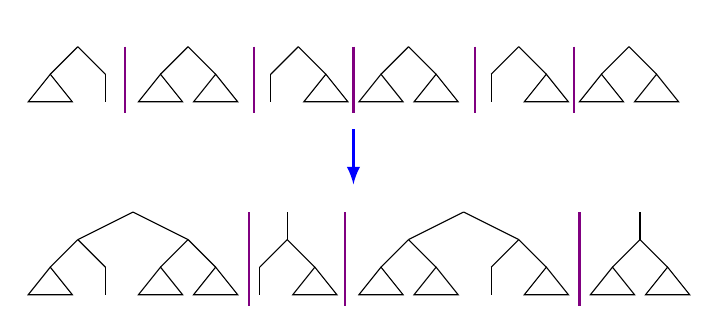
\begin{tikzpicture}[scale=0.7]

    \def\smallTriangle#1{
      \draw (#1)--+(-0.4,-0.5)--+(+0.4,-0.5)--cycle;
    }
    \def\smallEdge#1{
      \draw (#1)--+(-0,-0.5);
    }
    
    
    \def\leftTree#1#2#3#4{
        \begin{scope}[shift={#2}]
        \node[above] at (0,0) {#1};
        \draw (0,0)--(-0.5,-0.5);
        \draw (0,0)--(0.5,-0.5);
        \ifx&#3&\smallEdge{-0.5,-0.5}  
        \else
            \smallTriangle{-0.5,-0.5}
        \fi
        \ifx&#4&\smallEdge{0.5,-0.5}  
        \else
            \smallTriangle{0.5,-0.5}
        \fi
        \end{scope}
    }
    
    \draw[very thick,-latex, blue] (5,-1.5)--+(0,-1);
    
    
    \begin{scope}
        \foreach \x in {0.85,3.2,5,7.2,9} {
        \draw[thick,violet] (\x,0)--+(0,-1.2);
        }
        \leftTree{}{(0,0)}{x}{}
        \leftTree{}{(2,0)}{x}{x}
        \leftTree{}{(4,0)}{}{x}
        \leftTree{}{(6,0)}{x}{x}
        \leftTree{}{(8,0)}{}{x}
        \leftTree{}{(10,0)}{x}{x}
    \end{scope}
    
    \begin{scope}[xshift=1cm,yshift=-3cm]
        \foreach \x in {2.1, 3.85, 8.1} {
        \draw[thick,violet] (\x,0)--+(0,-1.7);
        }
        
        \begin{scope}[xshift=0cm]
        \node[above] at (0,0) {};
        \draw(0,0)--(-1,-0.5);
        \draw(0,0)--(1,-0.5);
        \leftTree{}{(-1,-0.5)}{x}{}
        \leftTree{}{(1,-0.5)}{x}{x}
        \end{scope}
        
        \begin{scope}[xshift=2.8cm]
        \node[above] at (0,0) {};
        \draw(0,0)--(0,-0.5);
        \leftTree{}{(0,-0.5)}{}{x}
        \end{scope}
        
        \begin{scope}[xshift=6cm]
        \node[above] at (0,0) {};
        \draw(0,0)--(-1,-0.5);
        \draw(0,0)--(1,-0.5);
        \leftTree{}{(-1,-0.5)}{x}{x}
        \leftTree{}{(1,-0.5)}{}{x}
        \end{scope}
        
        \begin{scope}[xshift=9.2cm]
        \node[above] at (0,0) {};
        \draw(0,0)--(0,-0.5);
        \leftTree{}{(0,-0.5)}{x}{x}
        \end{scope}
    
    \end{scope}
    
\end{tikzpicture}
   \caption{
  Schematic view of one iteration of restricted recompression
  (with phrase boundaries indicated).}\label{fig:schematic}
\end{figure}

Next, we describe operations being the basic building blocks of restricted recompression.
They are modifications of operations used in standard recompression~\cite{DBLP:journals/jacm/Jez16}.

\begin{definition}[{\bf Restricted run-length encoding}]\label{it:rle}Given a string  and a subset , we define an operation  that returns a string in  as shown in \cref{algo:RLE}.

\begin{minipage}[t]{.93\textwidth}\vspace{0pt}
\begin{algorithm}[H]
\ForEach{maximal unary run  \KwSty{in}  with  and }{replace  with ;}
\Return{}\;
\caption{}\label{algo:RLE}
\end{algorithm}
\end{minipage}
\end{definition}

\begin{definition}[{\bf Restricted pair compression}]\label{it:pair}
Given a string  and disjoint subsets , we define an operation
 that returns a string in  as shown in \cref{algo:PC}.

\begin{minipage}[t]{.93\textwidth}\vspace{0pt}
\begin{algorithm}[H]
\ForEach{fragment  \KwSty{in}  with  and }{
replace  with \;
}
\Return{}\;
\caption{}\label{algo:PC}
\end{algorithm}
\end{minipage}
\end{definition}


\begin{figure}[h]
\centering
\begin{center}
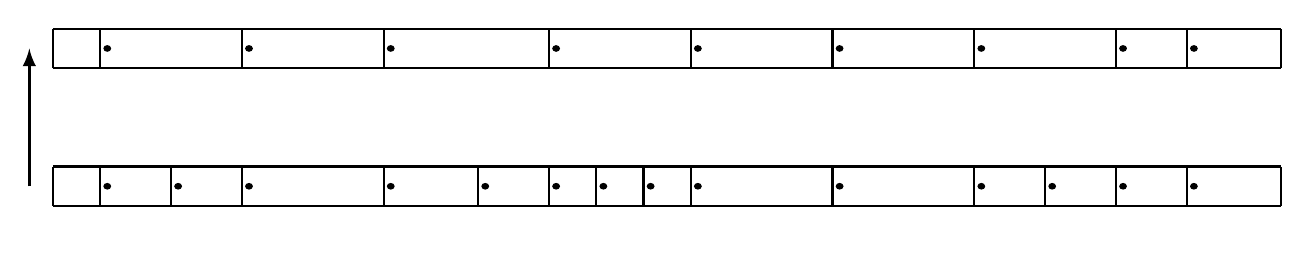
\begin{tikzpicture}[xscale=0.6,yscale=0.5]\foreach \x in {0,1,2.5,4,7,9,10.5,11.5,12.5,13.5,16.5,19.5,21,22.5,24,26}{
  \draw[thick] (\x,0) -- (\x,1);
}
\foreach \x/\j in {1/1,2.5/2,4/3,7/4,9/5,10.5/6,11.5/7,12.5/8,13.5/9,16.5/10,19.5/11,21/12,22.5/13,24/14}{
  \draw[xshift=0.15cm] (\x,0) node[below] {};
  \filldraw[xshift=0.15cm] (\x,0.5) circle (0.07cm);
}
\foreach \x/\c in {0.5/D,1.75/A,3.25/B,5.5/E,8/C,9.75/B,11/D,12/D,13/D,15/E,18/E,20.25/A,21.75/B,23.25/A,25/C}{
  \draw (\x,0.5) node {};
}
\draw[thick] (0,0) -- (26,0)  (0,1) -- (26,1);

\draw[very thick,-latex] (-0.5,0.5) -- (-0.5,4);

\begin{scope}[yshift=3.5cm]
\foreach \x in {0,1,4,7,10.5,13.5,16.5,19.5,22.5,24,26}{
  \draw[thick] (\x,0) -- (\x,1);
}
\foreach \x/\j in {1/1,4/3,7/4,10.5/6,13.5/9,16.5/10,19.5/11,22.5/13,24/14}{
  \draw[xshift=0.15cm] (\x,0) node[below] {};
  \filldraw[xshift=0.15cm] (\x,0.5) circle (0.07cm);
}
\foreach \x/\c in {0.5/D,5.5/E,15/E,18/E,23.25/A,25/C}{
  \draw (\x,0.5) node {};
}
\draw (2.5,0.5) node {};
\draw (8.875,0.5) node {};
\draw (12,0.5) node {};
\draw (21,0.5) node {};
\draw[thick] (0,0) -- (26,0)  (0,1) -- (26,1);
\end{scope}
\end{tikzpicture}
\end{center}
 \caption{Detailed illustration of one iteration of computing the
restricted recompression,
moving from 
to .
The dots correspond to phrase boundaries.
The set of phrase boundaries is changed as follows: .
We have  and . Further, , so  is not shrunk.}\label{fig:parse}
\end{figure}


\begin{definition}[{\bf Restricted recompression}]\label{constr:Jez}
Given a string , the strings  for  are constructed as shown in \cref{algo:RECOMPR}; see also \cref{fig:parse}.

\begin{minipage}[t]{.93\textwidth}\vspace{0pt}
\begin{algorithm}[H]
;\ \ \;
\While{}{
  \;
  \;
  \;
  \;
  , where  are disjoint subsets of  specified later\;
  \;
}
;
\caption{Constructing  restricted recompression
}
\label{algo:RECOMPR}\mbox{ \ }\\
\end{algorithm}
\end{minipage}
\end{definition}

\subsection{Efficient Implementation of Restricted Recompression}
Before we proceed with an efficient construction algorithm, let us show two basic properties of restricted recompression.
We view each application of a shrinking method ( or ) in \cref{algo:RECOMPR} as a decomposition of  into fragments, called \emph{blocks},
such that single-character blocks stay intact, and longer blocks are \emph{collapsed} into single characters in .
We refer to \emph{block boundaries} as positions of  where blocks start.

A distinctive feature of recompression (compared to other locally consistent parsing techniques)
is that matching phrases are given equal names.
More generally, the following property is shown by induction.

\begin{lemma}\label{fct:cons}
For every  and fragments  of , if the fragments expand to equal strings, that is ,
then  and  are formed of the same sequences of phrase names, that is .
\end{lemma} 
\begin{proof}
We proceed by induction on . 
Let  be fragments of  satisfying .
If , then  holds due to  and .
Otherwise, let  and  be the fragments of  obtained from  and , respectively, by expanding collapsed blocks.

Note that , so the inductive assumption guarantees .
Inspecting \cref{it:rle,it:pair}, we can observe that if  for ,
then block boundaries at positions  and  are placed consistently, that is,
either at both of them or at neither of them.
Consequently, block boundaries within  and  are placed consistently.
Moreover, both  and  consist of full blocks (since they are collapsed to  and , respectively). Thus,  and  are consistently partitioned into blocks. 
Matching blocks get collapsed to matching symbols both in \cref{it:rle,it:pair}, so we derive .
\end{proof}

In particular, we conclude that  holds for all odd .
\begin{corollary}\label{cor:distinct}
  For every odd , there is no  such that .
  \end{corollary}
  \begin{proof}
    For a proof by contradiction, suppose that  holds for some .
    By the definition of , we have .
  Let  be 
blocks of  collapsed to  and , respectively. 

Due to , \cref{fct:cons} guarantees  and, in particular, .
    If , then 
Otherwise,  for some symbol ,
    which means that .

In either case, , which means that  does not place a block
    boundary at position  in , a contradiction.
  \end{proof}


The classification into left and right symbols is made similarly as in~\cite[Lemma 6.2]{DBLP:journals/talg/Jez15}.
We formulate an auxiliary problem and use its folklore deterministic linear-time solution employing the so-called method of conditional expectations~\cite[Section 6.3]{MU05}.
A proof of the following lemma is provided in \cref{app:AMDC} for completeness.

\defdsproblem{\textsc{Approximate Maximum Directed Cut}}{
\textbf{Input}: A directed multigraph  without self-loops.\\
\textbf{Output}:
A partition  such that at least  arcs lead from  to .
}

\begin{restatable}{lemma}{AMDC}
\label{lem:maxcut}
The \textsc{Approximate Maximum Directed Cut} problem can be solved in  time.
\end{restatable}

We are ready to provide a deterministic algorithm for computing phrase boundaries of restricted recompression, shown in the proposition below.
It implies, in particular, that  is empty for appropriately large , so the number of iterations 
of the restricted recompression is .

In the implementation of operation  in restricted recompression, we construct a multigraph with vertices
, such that there is an arc from  to  for  if both symbols belong to , i.e., both  and  have lengths at most .
The sets  are the output  of the \textsc{Approximate Maximum Directed Cut} on this multigraph.
The number of arcs from  to  is exactly the number of pairs of collapsed blocks; the fact that it is bounded from below
guarantees that  decreases exponentially.
The steps using  do not need to reduce the number of phrases, but they guarantee that there are no self-loops in the constructed multigraphs
(cf.\ \cref{cor:distinct}).

\begin{proposition}\label{lem:recompr2}
  Given a string , a family
  of phrase boundaries  representing a restricted recompression  can be constructed in  time,
  with an extra guarantee that  holds for .
\end{proposition}
\begin{proof}
For subsequent integers , we represent the symbols of  via \emph{identifier functions} 
mapping distinct symbols to distinct identifiers in .
Thus, we actually store strings  such that  and  for .
Moreover, we store arrays mapping identifiers to expansion lengths of 
the corresponding symbols: . 

From this representation, it is easy to derive the equality

In order to construct  and , we sort the characters of  and assign them consecutive positive integer identifiers;
the lengths are obviously  for all .
This step takes  time due to the assumption .
Moreover,  holds as claimed.

In order to construct  and  for , we process  and 
depending on the parity of .

\paragraph{Case 1:}  is even, that is, .

We scan  from left to right outputting representations of subsequent symbols of .
The representations are elements of ; later, they will be given identifiers in .
Each symbol  in  is represented as , such that , , and  does not occur in , or as  otherwise.
Suppose that  is yet to be processed.
If 
we output  as the next symbol of  and continue processing .

Otherwise, we determine the maximum integer  such that  for ,
output  as the next symbol of , and continue processing .
By \cref{fct:cons},  does not occur in  in this case.

Note that . The characters of  are initially represented as elements of . Thus, these characters can be sorted in  time so that consecutive integer identifiers  are assigned to symbols of . 

We also set 
\begin{itemize}
\item 
 if  is represented as  and 

\item  if  is represented as .
\end{itemize}

Overall, this algorithm constructs  in  time.
Note that, by the inductive assumption,


\paragraph{Case 2:}  is odd, that is, .

We first partition  into  and .
Technically, this step results in appropriately marking  depending on whether ,
, or .

For this, we scan the array  and construct a directed multigraph  with .
For each , we add an arc 
provided that 


By \cref{cor:distinct}, this arc is not a self-loop,
so the algorithm of \cref{lem:maxcut} yields in  time a partition  with at least 
arcs from  to . For all symbols  such that , if , then we add  to ,
and otherwise we add it to .

Next, we scan  from left to right outputting representations of subsequent symbols of .
Initially, each symbol  in  is represented as , such that  and  does not occur in , or as  otherwise.
Suppose now that  is yet to be processed.
 If
 
we output  as the next symbol of  and continue processing 
the fragment .

Otherwise, we output  as the next symbol of  and continue processing .
By \cref{fct:cons},  does not occur in  in this case.

Note that  and that the characters of  are initially represented as elements of .
Thus, these characters can be sorted in  time so that consecutive integer identifiers  can be assigned to symbols of . 

We also set 

\begin{itemize}
\item
 if  is represented as  and 

\item
 if  is represented as .
\end{itemize}

Overall, this algorithm constructs  in  time.
Moreover, we have  by construction of the partition .

Observe that, for , an arc   is not added to  
only if 
 or .
There are at most  indices  such that  and each of them prevents at most two arcs from being added to .
Thus, , and consequently 


The algorithm terminates after constructing the first string  with  and even  (then,  for ). The overall running time is 

\end{proof}

\subsection{Properties of Restricted Recompression}
Restricted recompression guarantees that phrase lengths can be bounded as shown in the following fact.
\begin{fact}\label{fct:recompr}
For every  and every symbol  occurring in , the expansion  has length at most  or primitive root of length at most .
\end{fact}
\begin{proof}
  We proceed by induction on . 
  Let  be a symbol in . If , then .
  Thus, we may assume .

  If  also occurs in ,
  then the inductive assumption shows that  
  is of length at most 
  or its primitive root is of length at most . 
  
Otherwise, we have two possibilities.
  If  is odd, then ,
  and thus the primitive root of  is of length at most .
  If  is even, on the other hand, then ,
  so .
\end{proof}

What is even more important, restricted recompression guarantees that the sets  are locally consistent.
\lemcons*
\begin{proof}
  We proceed by induction on . The base case of  is trivially satisfied
  due to .
  
  Let .
  For a proof by contradiction, suppose that 
  By  and the inductive assumption,  implies .
  
  Let us set  so that
   and  are the first positions of the phrases induced by  and , respectively,
  that is,  and .
  Since a block boundary was not placed at ,
  we have  (see \cref{it:rle,it:pair}). 
  Therefore, the phrases  and  around position  are of length at most . 
  
  Since , by the inductive assumption,  and  imply  and , respectively.
  Due to \cref{fct:cons}, this yields 
  
  Consequently, a block boundary was not placed at ,
  which contradicts .
\end{proof}


Finally, let us show that the elements of the sequence  are bounded by the elements of the sequence  as follows.
\begin{observation}\label{obs:d_alpha}
For every , we have .
\end{observation}
\begin{proof}
We denote  and observe that
 
\end{proof}

\section{Details of the Synchronizing Sets Hierarchy Construction}\label{sec:correctness}

In this section, we use the properties of the hierarchy of phrase boundaries  and those of the family  of -runs to prove that \cref{def:syncfr} yields synchronizing sets of desired size. Moreover, we show how to efficiently build these synchronizing sets.

\begin{lemma}\label{lem:sss}
Let  be as in \cref{def:syncfr} for a given .
Then,  is a -synchronizing set of size .
\end{lemma}
\begin{proof}
We prove that  satisfies the two conditions of \cref{def:sss} and analyze the size of .

\paragraph*{\bf Consistency:}
Suppose that two length- fragments  and  satisfy  and .
We will show that if  satisfies condition~\ref{it:a}--\ref{it:c} in \cref{def:syncfr}, then  satisfies the same condition and .

If  satisfies condition~\ref{it:a}, then , and we need to prove that . This statement is trivial if  due to . Otherwise, the statement holds due to \cref{lem:cons} applied for  because  holds by \cref{obs:d_alpha}, and hence . Moreover, if  is -non-periodic, then so is .

By the next claim, in conditions~\ref{it:b} and~\ref{it:c} of \cref{def:syncfr}, we do not need to explicitly mention that the respective synchronizing fragment is -non-periodic. The claim follows from~\cref{fct:uni}.

\begin{claim}\label{fct:bc}
If the first (last) position of a length- fragment of  is one position to the left (right, respectively) of a -run, then the fragment is -non-periodic.
\end{claim}

If  satisfies condition~\ref{it:b}, then

so there is a -run extending the fragment  to the right in ; therefore,  satisfies condition~\ref{it:b} and 
(cf.~\cref{fct:bc}).

Condition~\ref{it:c} is symmetric to condition~\ref{it:b}; in this case, there is a -run extending the fragment  to the left in .

\paragraph*{\bf Density:}
Consider a position .
We first show that if , then .

We start by identifying  a -run  with

First, suppose that there exists a position .
Then,  since otherwise  would have been added to  by condition~\ref{it:a},
and thus  would have been added to .
Hence, the run  starts at position  and ends at position .

Next, suppose that .
Then,  is contained in a single phrase of~.
The length of this phrase is at least .
If , then  contradicts the fact that all phrases in  are of length .
Otherwise, , so \cref{fct:recompr} yields 

Now, the -run  satisfies the desired requirement.

Note that the fragments  and  satisfy conditions~\ref{it:b} and~\ref{it:c}, respectively (cf.\ \cref{fct:bc}).
Due to , this implies  and ,
which means that  holds as claimed.

\medskip
It remains to show, for all , that
if , then ;
equivalently, we need to argue that if , then .
Indeed, if ,
then  

\paragraph*{\bf Size:}
Observe that . 
The second term can be bounded using \cref{fct:uni}:
\begin{claim}
  .
\end{claim}
\begin{proof}
  By \cref{fct:uni}, distinct -runs  satisfy .
  Consequently, each -run  contains more than 
  (trailing) positions which are disjoint from all -runs starting to the left of .
\end{proof}
As for , we rely on the upper bound of \cref{lem:recompr2}
and note that  holds by the definition of .
Hence,

\end{proof}

Before we provide an implementation of \cref{def:syncfr}, we need to make sure that the sets  can be built efficiently.
\begin{lemma}\label{lem:tauruns}
  After -time preprocessing of a text  of length ,
  given an integer , 
  one can construct in  time the set  (with runs ordered by their start positions). 
\end{lemma}
\begin{proof}
  For every , let us define 
  
  By \cref{fct:uni}, distinct runs  satisfy ,
  and therefore .
  Moreover, note that  holds for  due to
  
 
  \paragraph{\bf Preprocessing.}  In the preprocessing phase, the algorithm computes the values  for 
  and the sets  for ,
  with runs ordered by their start positions.
  In order to construct the sets , the algorithm builds  using \cref{fct:runs}
  and sorts the runs in  according to their start positions using bucket sort.
  Then, each  is added to the appropriate sets ,
  i.e., whenever .
  The preprocessing time is therefore .
\paragraph{\bf Queries.}  At query time, given an integer , the algorithm retrieves 
  and iterates over , outputting  whenever .
  The correctness follows from  , and the query time is  due to .
\end{proof}

We are ready to prove the main result of this section, that is, -time construction of a data structure that allows computing
a -synchronizing set in time , for any .

\thmsss*
\begin{proof}
  In the preprocessing phase, the algorithm constructs the sets  using \cref{lem:recompr2},
  performs the preprocessing of \cref{lem:tauruns},
  and computes
   for all .

  The query algorithm follows \cref{def:syncfr}. Synchronizing fragments satisfying conditions~\ref{it:a}--\ref{it:c}
  are constructed independently (in the left-to-right order) and then the three sorted lists are merged.
  The construction of all three lists relies on the list  of -runs obtained from \cref{lem:tauruns}. The list is sorted by start positions, but since no -run is contained within another -run, also by end positions.

  The synchronizing positions satisfying condition~\ref{it:a} are  for each  such that  is not contained in any -run,
  i.e., 
  To check this condition, the algorithm simultaneously iterates over positions in  and 
  the list .

  The positions satisfying condition~\ref{it:b} are  for every  with .
  (Recall \cref{fct:bc}.)
  Thus, they can be generated by iterating over the list .

  Finally, the positions satisfying condition~\ref{it:c} are  for every  with .
  Thus, they can be generated by iterating over the list .

  Overall, constructing  costs  time.
  As observed in the proof of \cref{lem:sss}, each of these terms can be bounded by .
  Finally, the same lemma guarantees that  is a -synchronizing set of size .
\end{proof}

\section{\IPM with -Patterns}\label{chp:ipm}
\newcommand{\rx}{\hat{x}}

As discussed in \cref{sec:techniques}, in order to support \IPM in the text~, we use a classic idea of pattern matching by deterministic sampling~\cite{DBLP:journals/siamcomp/Vishkin91} in a novel way.
The main trick is to select a consistent family  of \emph{samples}.
This allows answering \emph{restricted} \IPM, with , using a relatively simple approach
in  space; see \cref{sec:impl}.


\begin{figure}[h]
  \begin{center}
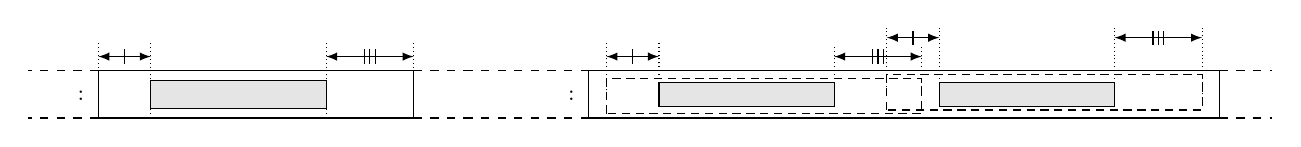
\begin{tikzpicture}[xscale=.445,yscale=.6,font=\footnotesize]
\draw (3.5,0) rectangle (12.5, 1);
\draw[dashed] (3.5, 0) -- (1.5,0);
\draw[dashed] (3.5, 1) -- (1.5,1);
\draw[dashed] (12.5, 0) -- (14,0);
\draw[dashed] (12.5, 1) -- (14,1);


\draw (3, .5) node[anchor=mid] {:};

\draw[fill=black!10] (5, .2) rectangle  (10, .8);
\draw (7.5, 0.5) node[anchor=mid]{\scriptsize };

\draw[latex-latex] (12.5, 1.3) --  (10, 1.3);
\draw[latex-latex] (3.5, 1.3) --  (5, 1.3);

\foreach \x in {4.25, 11.1, 11.25,11.4}
	\draw (\x,1.15) -- (\x,1.45);

\draw[densely dotted] (3.5, 0) -- (3.5, 1.6);
\draw[densely dotted] (5, 0) -- (5, 1.6);
\draw[densely dotted] (10, 0) -- (10, 1.6);
\draw[densely dotted] (12.5, 0) -- (12.5, 1.6);


\begin{scope}[xshift = 14cm]
\draw (3.5,0) rectangle (21.5, 1);
\draw[dashed] (3.5, 0) -- (0,0);
\draw[dashed] (3.5, 1) -- (0,1);
\draw[dashed] (12.5, 0) -- (23,0);
\draw[dashed] (12.5, 1) -- (23,1);


\draw (3, .5) node[anchor=mid] {:};

\foreach \x/\y in {4/0.09, 12/0.17} {
\draw[fill=black!10] (\x+1.5, .25) rectangle  (\x+6.5, .75);
\draw[densely dashed] (\x, \y) rectangle (\x+9, \y+0.75);
\draw[densely dotted] (\x, 0.5) -- (\x, 1.6);
\draw[densely dotted] (\x+1.5, 0.5) -- (\x+1.5, 1.6);
}

\foreach \x/\y in {4/1.3, 12/1.7}{
\foreach \z in {\x, \x+1.5, \x+6.5, \x+9}{
	\draw[densely dotted] (\z, 0.5) -- (\z, \y+0.2);
}

\draw[latex-latex] (\x, \y) --  (\x+1.5, \y);
\draw[latex-latex] (\x+9, \y) --  (\x+6.5, \y);
\foreach \z in {\x+0.75, \x+7.6, \x+7.75,\x+7.9}{
	\draw (\z,\y-0.15) -- (\z,\y+0.15);
}
}




\end{scope}
\end{tikzpicture}
\end{center}
   \caption{\label{fig:repr}
  The main idea of the query algorithm for fragments  and .
  We find the occurrences of  contained in  (depicted as gray rectangles).
  If there is an occurrence  of  contained in , then 
  can be obtained by extending an occurrence of  within .
  Hence,  must be one of the fragments marked with dashed rectangles. 
  }
  \end{figure}

In the general case, we first select an arbitrary sample  contained in 
and search for the occurrences of  within . 
Then, our query algorithm checks which occurrences of  can be extended to occurrences of ; see \cref{fig:repr}.
In order to achieve constant query time with this approach, we need to guarantee that  has   occurrences in . 
In general, already  might have  occurrences within .
Nevertheless, the following observation can be applied to bound the number of occurrences provided that  does not have a short period.
In particular, if  and , then  has at most three occurrences within~.

\begin{fact}[Sparsity of occurrences]\label{fct:far}
  If a substring  occurs in a text  at distinct positions , then .
  \end{fact}
  \begin{proof}
  If  with , then  for every , i.e.,  is a period of .
  \end{proof}



\subsection{Selection of Samples}\label{sec:repr}
Let us start with a formal definition based on the discussion above.
\begin{definition}\label{def:repr}
  A family  of fragments of  is a \emph{samples family} if it satisfies the following conditions:
  \begin{enumerate}[label=(\alph*)]
    \item\label{it:repr:cons} For all fragments  of , if  and , then .

\smallskip
    \item\label{it:repr:dens} For every , there exists a fragment  contained in  such that .
  \end{enumerate}
\end{definition}

Let us first analyze simple ways to select samples. 
Arguably, the most naive choice is .
In this case, the correctness is obvious, with each  being its own sample.
However, the number of samples can only be bounded by .

An easy way to dramatically reduce the number of samples is to set  so that . 
Then, as a sample of , we can select an arbitrary fragment 
of length  contained in . 
By the following result, such a fragment always exists.
\begin{fact}\label{fct:nonp}
  For every fragment  and length ,
  there is a fragment  of length  contained in .
  \end{fact}
  \begin{proof}
  Suppose that .
  Then, there exists a run  with . 
  Hence,  is a proper prefix of ,
  i.e.,  for some .
  We then define .
  If , then there would be another run  in  with .
  Now,  contradicts  \cref{fct:uni}.
  \end{proof}

We aim to select just  samples.
For this, we use synchronizing sets of \cref{thm:sss}.
\begin{lemma}\label{lem:repr}
The family ,
where  is the set of -synchronizing fragments of \cref{thm:sss}, satisfies \cref{def:repr}.
\end{lemma}
\begin{proof}
Let  denote the -synchronizing set containing starting positions of fragments in .
The consistency property~\ref{it:repr:cons} follows immediately from the 
corresponding property of synchronizing sets.

As for the existence of samples (property~\ref{it:repr:dens}),
let us fix  and choose 
so that .

If , then , so  can be chosen as its own sample.

Otherwise, let  be a fragment contained in  such that ; such a fragment  exists due to \cref{fct:nonp}.
Observe that 

Let ; by \cref{def:sss}, ,
so we select an arbitrary fragment  with  as the sample of .
Note that  is contained in  and  is contained in .
Moreover, 
by the extra condition of \cref{thm:sss}, and thus  holds as required.
\end{proof}

We conclude with an algorithmic construction based on \cref{lem:repr}.
\begin{proposition}\label{prp:repr}
Given a text  of length , one can in  time construct
a samples family  along with a data structure that,
given a fragment ,
  in  time reports a sample  contained in  and satisfying .
Moreover, for each , we have .
\end{proposition}
\begin{proof}
The construction builds -synchronizing sets 
for  and the family  as specified in \cref{lem:repr}.
The synchronizing sets are built using \cref{thm:sss}, which gives .
Moreover, the construction time is .
For every , the number of samples of length  or more
is  as claimed.

It remains to efficiently implement assigning samples
to fragments , following the approach described in the proof of \cref{lem:repr}.

The case of , when  is its own sample, does not require any infrastructure. 

To efficiently find samples for 
and , we
store  for each position  divisible by .
The size and construction time of this component is ,
which is  in total across all values of .

A query for a sample of  is answered as follows. 
As described in the proof of \cref{lem:repr}, we have . 
Moreover,  also yields 

Consequently, 
or  , and the underlying fragment can be reported 
as the sample of .
The query time is constant.
\end{proof}

\subsection{Implementation of the Data Structure}\label{sec:impl}
As outlined at the beginning of this section, to search for the occurrences of  in , we first find
in  the  occurrences of the sample  of .
This step is implemented using auxiliary \RIPM specified below.
Next, we apply \LCEQ (see \cref{prop:lce}) to check which occurrences of  can be extended to occurrences of ;
see also \cref{fig:repr}.

\defdsproblem{\RIPM}{
\textbf{Input}: A text  and a family  of fragments of .\\
\textbf{Queries}: Given a fragment  and a fragment  of , report all fragments 
contained in  and matching .
}

Due to the sparsity of occurrences (\cref{fct:far}),
it is relatively easy to implement \RIPM in  time using static dictionaries.

\begin{lemma}\label{lem:locator}
For any family  of fragments of a length- text , there exists a data structure of size 
that answers \RIPM in  time. It can be constructed in  time
in general and in  time if  for each , where  is the machine word size.
\end{lemma}
\begin{proof}
Given the family , we construct an identifier function  such that  if and only if the fragments  match.
For this, we order the fragments  by the length  and the lexicographic rank of the suffix  among the suffixes of  (this rank is the th entry of the inverse suffix array of , which can be built in  time~\cite{DBLP:journals/jacm/KarkkainenSB06}).
Matching fragments  appear consecutively in this order, so we use \LCEQ (see~\cref{prop:lce}) to determine the boundaries between the equivalence classes.

We store two collections of dictionaries.
The first collection allows converting samples to identifiers.
The second collection stores non-empty answers to selected \RIPM.

\paragraph{Dictionaries of identifiers.}
We store the  function in multiple static dictionaries jointly mapping each fragment   to the identifier .
Specifically, for each position  in , we store a dictionary  mapping  to 
for every fragment . 

In the general case, we use deterministic dictionaries by Ružić~\cite{DBLP:conf/icalp/Ruzic08},
which provide  query time, take  space, and have 
construction time, where  is the dictionary size. 
Across all positions , this brings the overall space consumption to  and the overall construction time to .
In case of short fragments , we use fusion trees~\cite{DBLP:conf/focs/PatrascuT14},
which provide  query time, take  space, and require 
construction time. Since the number of fragments in 
starting at any given position  is  in this case, this brings the overall space consumption and
the overall construction time to , whereas the query time is .

\paragraph{Dictionaries of answers to selected queries.}
For each , we cover the text  with blocks (fragments) of length  with overlaps of length  (the last block can be shorter)
and denote the resulting family of blocks by .
We store the non-empty answers to \RIPM for  and  in multiple static dictionaries.
Specifically, for each integer  and each fragment ,
we store a dictionary .
For each sample  that is contained in  and satisfies ,
the dictionary  maps the identifier  to the answer to a \RIPMOne for  and .
Note that each fragment  is contained in one or two blocks , 
so each  appears in  precomputed answers, and thus the total number of dictionary entries is .

In the general case, we use deterministic dictionaries by Ružić~\cite{DBLP:conf/icalp/Ruzic08},
which provide  query time, take  space in total, and have  
overall construction time.
In case of short patterns, we use fusion trees~\cite{DBLP:conf/focs/PatrascuT14},
which provide  query time, take  space in total, and have  construction time,
since each individual dictionary is of size  in this case (because each  contains  fragments  with ).

\paragraph{Query algorithm.}
To answer a query for  and , we first compute  and  using .
Next, we use simple arithmetics to obtain  blocks  
that collectively contain all length- fragments contained in .
We take the union of the precomputed answers for the identifier  in dictionaries  to obtain a collection of fragments  matching  and contained in one of the blocks .
By \cref{fct:far}, there are  such fragments , so we can filter and report those contained in  spending  time on each candidate .
\end{proof}

\begin{corollary}\label{cor:locator}
  Given the family  of samples of a length- text 
  constructed through \cref{prp:repr},
  one can in  time construct a data structure that answers \RIPM
  in  time.
\end{corollary}
\begin{proof}
We store two instances of the data structure of \cref{lem:locator}: the first instance,
for fragments of length more than , contains  samples,
and thus its construction time is .
The instance for the remaining fragments, of length at most , contains 
samples, and thus its construction time is also .
\end{proof}

We conclude with a full description of the data structure for \IPM for -patterns.
\begin{proposition}\label{prp:ipm}
  For every text  of length , there exists a data structure of size  which answers \IPM in  time provided that . The data structure can be constructed in  time.
\end{proposition}
\begin{proof}
  The core of our data structure is the samples family , constructed
  using \cref{prp:repr} along with a component for efficiently selecting a sample,
  plus the data structure answering \RIPM for , constructed using \cref{cor:locator}.
  Additionally, we include a data structure for \LCEQ (\cref{prop:lce}).
  Each of these ingredients takes  space and  time to build. 
  
  The query algorithm for fragments  and  works as follows.
  First, we use \cref{prp:repr} to obtain in  time a sample  contained in  and satisfying .
   Next, we query the component of \cref{cor:locator} to find all occurrences of  contained in ;
   this takes  time.
  As a result, we obtain a constant number of candidate positions where  may occur in .
  We verify them using \LCEQ in  time each.
  Recall that the occurrences of  in  form an arithmetic progression (\cref{fct:single}).
  \maybeqed \end{proof}

\section{\IPM with -Patterns}\label{chp:per}

Our approach to \IPM with -patterns relies on the structure of -runs in the text. In order to answer a query, we look for runs that may arise as  for the occurrences  of  within .
Due to the assumption , all these runs contain the middle position of   (the position  if  ).
All such runs need to have length at least  and period at most , which allows us to show that there are  such runs.
In \cref{sec:finder}, we develop a component listing such runs in  time after -time preprocessing.

 Next, we look for the occurrences of  contained in each candidate run .
 For  to have any occurrence in , the periods of  and  need to be equal;
 furthermore, the \emph{string periods} of  and ---that is, the prefixes of the two fragments of length equal to their periods---need to be cyclic rotations of each other.
 We then say that  and  are \emph{compatible}.
 To check this condition, we compare the lexicographically minimal rotations of the string periods, called \emph{Lyndon roots}.
 We use techniques originating from a paper by Crochemore et al.~\cite{DBLP:journals/tcs/CrochemoreIKRRW14}, listed in \cref{sec:comp},
 to check compatibility of substrings of  and list occurrences of an -pattern in a compatible -text;
 in this case, the set of occurrences forms an arithmetic progression.
 
 The query algorithm is described in \cref{sec:per_sum}.
 In brief, for each run  in  that is compatible with~, we can find all occurrences of  in  using the toolbox of~\cite{DBLP:journals/tcs/CrochemoreIKRRW14} (recalled in \cref{sec:comp}).
 We may obtain  arithmetic progressions representing the occurrences of  in ,
 but \cref{fct:single} guarantees that they can be merged into a single progression.


\subsection{Special -Runs}\label{sec:finder}
If  is an  fragment, then \cref{obs:char} yields the following useful characterization of .

\begin{observation}
Consider a text  and an -fragment  with . 
Then,  satisfies the following condition:

\end{observation} 

For a positive integer , we say that a run  is \emph{-special} if 
it satisfies condition \eqref{eq:obs:sprun} above.
Denote by  the set of -special runs covering position  in .
Below, we develop a data structure for efficiently answering the following queries:

\defdsproblem{\textsc{Special Run Locating Queries}}{
Given a position  of  and an integer , 
compute .
}

We first prove that the answers must be of constant size. Then, we develop a component for answering \textsc{Special Run Locating Queries} based on the fact that, even though there are  possible queries, it suffices to precompute answers to  of them.
\begin{lemma}\label{lem:atmost5}
 
for every integer  and position  in .
\end{lemma}
\begin{proof}
For a proof by contradiction, suppose that there are at least six such runs 
with  for  and .
For each , \cref{fct:uni} yields 

 so  is not contained in .
Observe also that .
Consequently, 

We derived , which contradicts .
\end{proof}



\begin{lemma}\label{lem:run_finder}
  For every text , there exists a data structure that answers \textsc{Special Run Locating Queries} in  time,
  takes  space, and can be constructed in  time.
\end{lemma}
\begin{proof}
  For every integer , the data structure contains the precomputed answers for all positions  divisible by .
  Each of these answers takes  space by \cref{lem:atmost5}, so the total size of the data structure is .

  As for the query algorithm, we note that if a -special run  covers position , then,
  due to , it also covers position  or .
  Thus, the query algorithm retrieves the answers for these two positions and, among the obtained -special runs,
  reports those covering position . The query time is constant by \cref{lem:atmost5}.

  As for the construction algorithm, we enumerate all runs using \cref{fct:runs}.
  For each -run  and each ,
  we append  to the precomputed answers for all positions  that are multiples of .
  Since there is at least one such position for each considered pair , the running time of this process
  is proportional to the time complexity of the algorithm of \cref{fct:runs} plus the total size of the precomputed answers, both of which are .
\end{proof}


\subsection{Compatibility of Strings and Runs}\label{sec:comp}
A primitive string  is called a \emph{Lyndon word}~\cite{Lyndon1954,chen1958free} if  for every rotation  of .
Let  be a string with the smallest period .
The \emph{Lyndon root}  of  is the lexicographically smallest rotation of the prefix .
We say that two strings are \emph{compatible} if they have the same Lyndon root.

A string  with Lyndon root  can be uniquely represented as , where  is a proper suffix of ,
  is a proper prefix of , and  is a non-negative integer.
The \emph{Lyndon signature} of  is defined as .
Note that the Lyndon signature uniquely determines  within its compatibility class.
This representation is very convenient for pattern matching if the text is compatible with the pattern.

\begin{lemma}\label{lem:lyndon}
Let  and  be compatible strings.
The set of positions where  occurs in  is an arithmetic progression that
can be computed in  time given the Lyndon signatures of  and .
\end{lemma}
\begin{proof}
Let  be the common Lyndon root of  and 
and let their Lyndon signatures be  and  respectively.
\cref{lem:synchr} (synchronization property) implies that  occurs in 
only at positions  such that .
Consequently,  occurs in  only at positions  such that .
Clearly,  occurs in  at all such positions  within the interval .
Therefore, it is a matter of simple calculations to compute the arithmetic progression of these positions.
\maybeqed \end{proof}

Crochemore et al.~\cite{DBLP:journals/tcs/CrochemoreIKRRW14} showed how to efficiently compute
Lyndon signatures of the runs of a~given~text.

\begin{fact}[Crochemore et al.~\cite{DBLP:journals/tcs/CrochemoreIKRRW14}]\label{fct:compat}
There exists an algorithm that, given a text  of length~, in  time
computes Lyndon signatures of all runs in .
\end{fact}

Finally, we note that the Lyndon signature of a periodic fragment  
can be derived from the Lyndon signature of .
\begin{observation}\label{obs:compat}
Let  be a fragment of a periodic string  such that  .
Then,  is compatible with .
Moreover, given the Lyndon signature of , one can compute the Lyndon signature of  in  time.
\end{observation}

\subsection{Answering Queries}\label{sec:per_sum}

Our data structure consists of the set of runs  (\cref{fct:runs}), with each run accompanied by its period and Lyndon signature (\cref{fct:compat}), the data structure for \LCEQ (\cref{prop:lce}), and the data structure of \cref{lem:run_finder} for \textsc{Special Run Locating Queries}.
The entire data structure takes  space and can be constructed in  time.

As outlined at the beginning of \cref{chp:per}, the query algorithm consists of the following steps:

\begin{center}
\begin{minipage}{14cm}
\noindent {\bf Algorithm} answering \IPM with -patterns

  \begin{enumerate}[label=(\Alph*)]
    \item\label{step:A} Compute the Lyndon signature of .
    \item\label{step:B} Find all -special runs  containing the middle position of ,
      defined as  for , along with their Lyndon signatures.
    \item\label{step:C} Filter out runs  incompatible with .
    \item\label{step:D}
	  For each of the compatible runs , compute an arithmetic progression representing the occurrences of  in .
	  \item\label{step:E}
      Combine the resulting occurrences of  in  into a single arithmetic progression.
  \end{enumerate}
  \end{minipage}
\end{center}

\paragraph*{Correctness.} Clearly, a fragment matching  (and contained in ) starts at each of the reported positions. 
It remains to prove that no occurrence  is missed.
Since , each occurrence  of  in  contains the middle point of .
Therefore,  is among the runs found in step~\ref{step:B}.
By \cref{obs:compat}, ~is compatible with  and, since  and  match,  must be compatible with . Hence,  is considered in step~\ref{step:D} and the starting position of  is reported in step~\ref{step:E}.

\paragraph*{Implementation.}
In step~\ref{step:A}, we use a \textsc{Special Run Locating Query} to list all -special runs containing the first position of , and then we check if any of these runs contains the whole  and has period not exceeding . If so, this run is  by \cref{obs:char}; otherwise, we raise an error to indicate that .
We then use \cref{fct:compat,obs:compat} to retrieve the Lyndon signature of  and , respectively.
In step~\ref{step:B}, we use another \textsc{Special Run Locating Query} to identify all  -special runs  containing the middle position of . \Cref{lem:atmost5} guarantees that we obtain at most five runs .
In step~\ref{step:C}, for each run , we use the Lyndon signatures 
to identify the Lyndon roots of  and , represented as fragments of ,
and we ask an \textsc{LCE Query} to check if the Lyndon roots match.

 For the remaining (compatible) runs , we apply \cref{lem:lyndon} to find the occurrences of  in .
 There is nothing to do if . 
Otherwise, , so \cref{obs:compat} lets us retrieve the Lyndon signature of .
 We are left with at most five arithmetic progressions, one for each compatible run .
 As argued above, their union represents all occurrences of  in .
 By \cref{fct:single}, this set must form a single arithmetic progression.
 If the progressions are stored by (at most) three elements---the last one and the first two---it is easy to compute the union in constant time.

The above query algorithm also checks if the fragment  is highly periodic. 
This concludes the proof of the following result:

\begin{proposition}\label{thm:per}
For every text  of length , there exists a data structure of size  which answers \IPM in  time provided that ,
and reports an error whenever .
The data structure can be constructed in  time.
\end{proposition}

Combining \cref{thm:per} with \cref{prp:ipm}, we obtain an efficient data structure for \IPM over integer alphabets of polynomial size.
\begin{theorem}\label{thm:ipm0}
  For every text  of length , there exists a data structure of size  which answers \IPM in  time.
  The data structure can be constructed in  time.
\end{theorem}

In the following section, we show how the data structure can be improved in the case of a small alphabet.

\section{\IPM in Texts over Small Alphabets}\label{sec:packed}
In this section, we assume that ; otherwise, \cref{thm:ipm} follows directly from \cref{thm:ipm0}.
We transform the string  into a string  of length , where .
Then, each \IPMOne in  is reduced to a constant number of \IPM in .
Without loss of generality, we assume that  starts and ends with unique characters to avoid degenerate cases.

A naive idea to construct the string  would be to partition  into blocks of length  and interpret each block as an integer with  bits.
Unfortunately, this approach is not helpful: even if a pattern fragment  has an occurrence in a text fragment  of ,
the longest fragment of  consisting of full blocks may have no ``aligned'' occurrence in the longest fragment of  consisting of full blocks.
Therefore, we partition the string into blocks using the elements of a -synchronizing set, which can be constructed in  time for the aforementioned value of ; see \cref{prp:synch}.

\subsection{Constructing Data Structure}
We use a -synchronizing set 
 of , where , and the corresponding set of synchronizing fragments , where
. 
The aforementioned assumption on  implies  and ; in particular, .

Denote  for .
We construct a length- string  such that 

Every character of  is either an integer in  or a length- substring of  (which can be interpreted as an integer with  bits); see \cref{fig:jak_chcesz}.


\begin{figure}[h]
  \centering
  \begin{tikzpicture}[xscale=0.63,yscale=0.74]
  \def\tauW{1.5}
  \def\perW{1.2}
  \def\boxH{0.5}

  \node at (0,0.5) [left] {};

  \def\curr{0}
  \foreach [count=\i]
    \w/\c
    in {1/A, 1/B, 2/C, 2/D, 2/C, 6/C, 4/D, 1/E} {
    \coordinate (l\i) at (\curr,0);
    \coordinate (b\i) at (\curr+\w,0);
    \coordinate (r\i) at (\curr+\w,0.8);
    \xdef\curr{\number\numexpr\curr+\w\relax}
  }
  \draw[thick] (l1) rectangle (r7) node[midway] {};  

  \begin{scope}[xshift=7cm,yshift=0.8cm]
    \clip (-\perW,0) rectangle (8.7,0.3);
    \foreach \dx in {0,...,10}{
      \coordinate (c\dx) at (\dx*\perW,0);
      \draw (\dx*\perW, 0) sin ((\dx*\perW+0.5*\perW, 0.3) cos ((\dx*\perW+1*\perW, 0);
    }
    \coordinate (b10) at ();
    \coordinate (b11) at ();
  \end{scope}


  \foreach \i/\y in {3/2, 2/1, 4/3} {
    \coordinate (bl\i) at ();
    \coordinate (bll\i) at ();
    \coordinate (br\i) at ();
    \coordinate (bc\i) at ();
    \coordinate (bu\i) at ();

    \draw[thin, blue, -latex] (bll\i) -- (l\i -| bll\i);

    \draw[fill=white] (bl\i) rectangle ();
  }

  \foreach \i/\y in {10/1, 11/2} {
    \coordinate (bl\i) at ();
    \coordinate (bll\i) at ();
    \coordinate (br\i) at ();
    \coordinate (bc\i) at ();
    \coordinate (bu\i) at ();

    \draw[thin, blue, -latex] (bll\i) -- (l1 -| bll\i);

    \draw[fill=white] (bl\i) rectangle ();
  }
  \draw[densely dotted] (br11)--();

  \node[blue, above] at (bll2 |- b1) {\small };
  \node[blue, above] at (bll3 |- b1) {\small };
  \node[blue, above] at (bll4 |- b1) {\small };
  \node[blue, above] at (bll10 |- b1) {\small };
  \node[blue, above] at (bll11 |- b1) {\small };

  \node[red, above] (j) at () {};
  \draw[violet,-latex, bend left=45] (j |- r1) to (bll4 |- r1);
  \node[above] at () {\small };


  \node[blue,yshift=0.17cm] at (bc2) {\small };
  \node[blue,yshift=0.17cm] at (bc3) {\small };
  \node[blue,yshift=0.17cm] at (bc4) {\small };
  \node[blue,yshift=0.17cm] at (bc10) {\small };
  \node[blue,yshift=0.16cm] at (bc11) {\small };


\begin{scope}[yshift=-4cm,xshift=-2cm]
\node at (0,0.05) {};
\foreach [count=\i] \l in {, , , , } {
  \coordinate (q\i) at (-3.2cm+4.2cm*\i,0);
  \draw () rectangle +(2*\tauW,\boxH) node[midway,blue] {\small \l};
}
\foreach [count=\i] \l in {\Delta_0, \Delta_1, \Delta_2, \Delta_3} {
  \node at () {\small };
}
\end{scope}

\end{tikzpicture}
   \caption{A schematic view of the transformation from  to , assuming  and .
  The  operation returns the index of the nearest synchronizing position if it exists; see below.}\label{fig:jak_chcesz}
\end{figure}

We say that a fragment of  is \emph{regular} if it is
of the form  for . For such a fragment , we denote the fragment .
\begin{fact}\label{fct:tp}
If  and  are regular fragments, then 
\end{fact}
\begin{proof}
Let  and  .

\paragraph*{(Implication )}
Suppose that .
We conclude from the consistency property of  that  and .
This implies that .
Hence,  holds as claimed.

\paragraph*{(Implication )}
Suppose that .
Equivalently, we have  and .
To obtain , we only need to show that if  holds for some ,  such that , then .
In this case, by the density property of , we have 
Since ,
\cref{obs:char} implies  and therefore .
As  also yields , this concludes the proof.
\end{proof}

Let  and  be sentinels. 
The sequence  of synchronizing positions
together with the sentinels partitions  into
intervals called \emph{blocks}: 

We define the following operation mapping each position  to the index of the block it belongs to;
see \cref{fig:jak_chcesz}:

We build a length- bitmask representing .
Then the  operation can be viewed as a  query on this bitmask.
These queries can be answered in  time using a data structure of size 
that can be constructed in  time~\cite{DBLP:conf/focs/Jacobson89,WaveletSuffixTree,DBLP:journals/tcs/MunroNV16}.

Recall that a run  is a -run if  and .
We say that a -run  is \emph{long} if  and use the following proposition for the considered .

\begin{proposition}[{\cite[Section 6.1.2]{Kempa2019}}]\label{prp:taurons}
For a positive integer , a string  contains  long -runs.
Moreover, if , we can compute all long -runs in
, compute their Lyndon signatures, and group the long -runs by their Lyndon roots in  time.
\end{proposition}

Let us note that a -run is -special.
Hence, each position in  belongs to at most five -runs (\cref{lem:atmost5}).
Moreover, we can locate long -runs using the same data structure as in \cref{lem:run_finder}, but constructed only for
 (and using \cref{prp:taurons} to compute all long -tuns):
\begin{lemma}\label{lem:run_finder2}
  For every text , there exists a data structure that can compute all long -runs containing a given position in  time,
  takes  space, and can be constructed in  time.
\end{lemma}

\noindent
We also perform preprocessing for \LCEQ (\cref{prop:lce}).

Finally, for every pair  of strings such that  and , we precompute
the set of occurrences of  in , represented as an arithmetic progression.
The total number of such pairs  is , and for each such pair,
the output can be computed in  time, so this preprocessing can be performed
in  time.


\subsection{Answering Queries} 
We denote by  the longest regular fragment 
contained in the fragment  of  and denote  .
Note that, for any two matching fragments , we have  (by consistency of )
and  (by \cref{fct:tp}); see \cref{fig:zz1}.

\begin{figure}[h]
 \centering
 \begin{tikzpicture}[xscale=1.2,yscale=1.2]
  \def\barW{1.0}
  
  \coordinate (l) at (0,0);
  \coordinate (lc) at (0, 0.2);
  \coordinate (r) at (10, 0.4);
  
  \node at () [right] {};
  
  \draw[thick] (l) rectangle (r);
  
  \coordinate (x) at ();
  \coordinate (xr) at ();
  \draw (x) rectangle (xr);
  \node at ([xshift=0.2cm,yshift=0.15cm]x) {};
  
  \coordinate (y) at ();
  \coordinate (yr) at ();
  \draw (y) rectangle (yr);
  \node at ([xshift=0.2cm,yshift=0.15cm]y) {};
  
  
  \foreach \dx/\dy [count=\i from 0] in {-0.1/0.5, 0.85/1, 2.0/1, 1.2/0.5, 2.6/0.5} {
    \coordinate (sl\i) at ();
    \coordinate (sr\i) at ();
    \coordinate (su\i) at (sl\i |- l);
  
    \draw[blue,fill=lightgray] (sl\i) rectangle (sr\i);
    \draw[blue] (sl\i)--(su\i);
  }
  \draw[blue,fill=black!10!white] (sl0) rectangle (sr0);
  \draw[blue,fill=black!10!white] (sl4) rectangle (sr4);

  
  \node at (su1) [blue, above] { };
  \node at (su2) [blue, above] {};
  



  \coordinate (zl) at (sl1 |- xr);
  \coordinate (zr) at ();
  \draw[densely dotted] (sl1)--(zl |- xr);
  \draw[densely dotted] (sr2)--(zr |- xr);
  \draw (zl) rectangle (zr);
  \node at ([xshift=0.2cm,yshift=0.15cm]zl) {};
  
  \coordinate (zc) at ();
  \draw[|<->|] (x |- zc)--(zc);
  
  
  \coordinate (y1) at (y |- l);
  \coordinate (y2) at ();
  \coordinate (y3) at ();


  \foreach \dx/\dy [count=\i] in {0.85/0.1, 2.0/0.1, 1.2/-0.35} {
    \coordinate (ssl\i) at ();
    \coordinate (ssr\i) at ();
  
    \draw[blue,fill=lightgray] (ssl\i) rectangle (ssr\i);
  }
  
  \node at (ssl1 |- ssr1) [above,yshift=0.03cm] { };
  \node at (ssl2 |- ssr2) [above] { };
  
  \coordinate (zzl) at ();
  \coordinate (zzr) at ();
  
  \coordinate (xxl) at ();
  \coordinate (xxr) at ();
  
  
  \draw (zzl) rectangle (zzr);
  \node at ([xshift=0.2cm,yshift=0.17cm]zzl) { };
  
  \draw[densely dotted] (ssl1) -- (zzl);
  \draw[densely dotted] (ssr2) -- (zzr);
  
  
  \draw (xxl) rectangle (xxr);
  \node at ([xshift=0.2cm,yshift=0.17cm]xxl) { };
  
  \coordinate (zzc) at ();
  \draw[|<->|] (xxl |- zzc)--(zzc);
  
  \end{tikzpicture}
  
  
  \caption{We have  and .
The arrows correspond to the same distances due to synchronization. Each fragment  matching  and contained in  determines a single location of a candidate match .}\label{fig:zz1}
\end{figure}

\begin{observation}
After -time preprocessing, given fragments ,  of ,
we can compute the fragments ,  in  and 
their codes ,  in  in  time.
\end{observation}

First, we consider the case when  and ; the remaining corner cases will be addressed later.
In \IPM, we assume that the length of  is proportional to the length of . 
Here, we will make a stronger assumption that . 
However, this assumption does not imply immediately that  is proportional to .
The latter condition is needed to apply \IPM to fragments  and  because  could be too large compared with .

Denote  and let  be the middle position of .
Our approach, in this case, is to restrict the search to 
an appropriate fragment of length at most ,

equal to an approximately the ``middle'' part of ; see \cref{new}.

\begin{figure}[h]
 \centering
 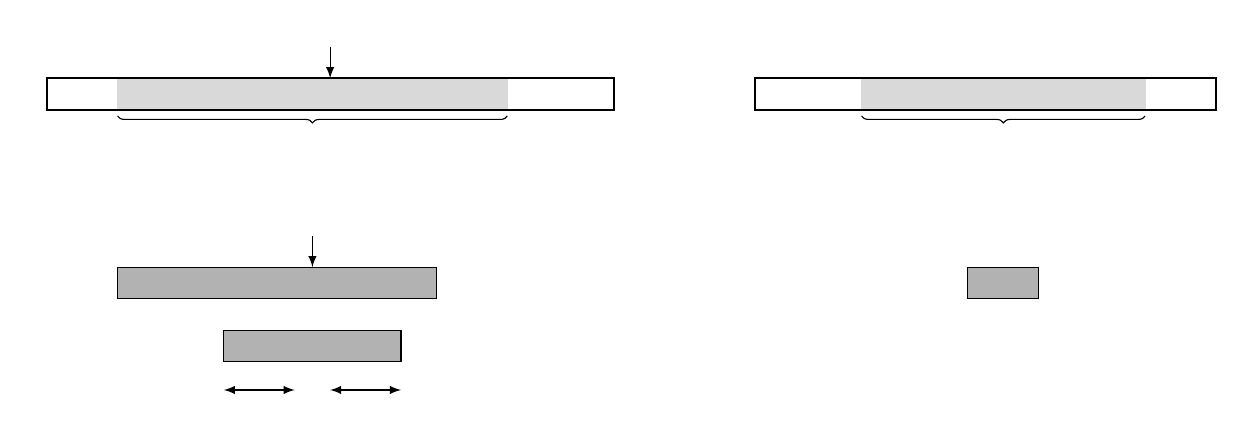
\begin{tikzpicture}[xscale=0.9,yscale=0.4]

\filldraw[white!85!black] (1,0) rectangle (6.5,1);
\draw[thick] (0,0) rectangle (8,1);
\draw (0,0.5) node[left] {};
\draw[-latex] (4,2) -- (4,1);
\draw (4,2) node[above] {};
\draw[snake=brace] (6.5,-0.2) -- node[below] {} (1,-0.2);

\begin{scope}[xshift=10cm]
\filldraw[white!85!black] (1.5,0) rectangle (5.5,1);
\draw[thick](0,0) rectangle (6.5,1);
\draw (0,0.5) node[left] {};
\draw[snake=brace] (5.5,-0.2) -- node[below] {} (1.5,-0.2);
\end{scope}

\begin{scope}[yshift=-6cm]
\begin{scope}[xshift=1cm]
\filldraw[white!70!black] (0,0) rectangle (4.5,1);
\draw (0,0) rectangle (4.5,1);
\draw (0,0.5) node[left] {};
\draw[-latex] (2.75,2) -- (2.75,1);
\draw (2.75,2) node[above] {};
\begin{scope}[yshift=-2cm]
\filldraw[white!70!black] (1.5,0) rectangle (4,1);
\draw (1.5,0.5) node[left] {};
\draw (1.5,0) rectangle (4,1);
\draw (2.75,0) node[below] {};
\draw[latex-latex] (1.5,-0.9) -- node[below] {} (2.5,-0.9);
\draw[latex-latex] (3,-0.9) -- node[below] {} (4,-0.9);
\end{scope}
\end{scope}
\begin{scope}[xshift=13cm]
\filldraw[white!70!black] (0,0) rectangle (1,1);
\draw (0,0) rectangle (1,1);
\draw (0.5,0) node[below] {};
\end{scope}
\end{scope}
  
\end{tikzpicture}  
  \caption{Instead of searching for  within , we only search within a fragment  of length at most .
 Recall that each character of  and  fits in a single machine word.
}\label{new}
\end{figure}

\begin{fact}\label{fct:easy}
Let  and  be fragments of  such that , and
let  be a fragment matching  and contained in .
If , then  contains  or , where .
\end{fact}
\begin{proof}
Recall that , so .
Let  so that .
It suffices to prove that .
\begin{itemize}
\item
If , then , so  and .

\smallskip
\item If , then, since both  and  are contained in ,
we conclude that  is contained in , contradicting the definition of .

\smallskip
\item Finally, if , then we claim that  is contained in ,
contradicting the definition of .
Indeed, ,
so  contains both  and ,
and thus also . \qedhere
\end{itemize}
\end{proof}

In the query algorithm below, we assume without loss of generality that .
(To handle , we combine the answers of up to four queries.)

\begin{center}
\begin{minipage}{14cm}
\noindent {\bf Algorithm} answering \IPM over small alphabets

  \begin{enumerate}[label=(\Alph*)]
    \item\label{Step:A} If , return a precomputed answer.
    \item\label{Step:B} If , apply the query algorithm for -patterns of \cref{sec:per_sum}.
    \item\label{Step:C} Apply \IPM for pattern  and text  (\cref{thm:ipm0}), obtaining
    at most two arithmetic progressions of occurrences.
    \item\label{Step:D} 
    Apply \cref{lem:peralg}\ref{it:permax} for  and  to test which of these occurrences extend to occurrences of .
  \end{enumerate}
  \end{minipage}
\end{center}

\paragraph*{Correctness.}
In step~\ref{Step:B}, if , then the density of  implies , so indeed  is an -pattern.

In step~\ref{Step:C}, we have , so \cref{fct:single} implies that there are up to two arithmetic progressions.

In step~\ref{Step:D}, we only care about occurrences of  starting at even positions of .
Each arithmetic progression from step~\ref{Step:C} forms a periodic progression  in~.
This is because, by \cref{fct:tp}, subsequent occurrences of  start at all these positions.
Let  and .
We apply \cref{lem:peralg}\ref{it:permax} in  to sequence , position , and fragment  to check which positions  contain occurrences of .
Then, we apply \cref{lem:peralg}\ref{it:permax} in  to sequence
, position , and fragment 
to check which positions  in  are endpoints of occurrences of .
In each case, the lemma returns an integer interval of indices.
The intersection of the two intervals can be transformed into an arithmetic progression of positions.
The two resulting arithmetic progressions can be joined together to one progression by \cref{fct:single}.

\paragraph*{Implementation.}
Recall that  is given in a packed representation.
In step~\ref{Step:A}, this lets us retrieve any fragment of length at most , encoded in a single machine word, in  time.
Then we can use the precomputed answer.

In step~\ref{Step:B}, the preprocessing of the query algorithm of \cref{sec:per_sum} takes only  time and space as we use \cref{lem:run_finder2} to find long -runs and the LCE queries of \cref{prop:lce}.

In step~\ref{Step:C}, we have  and  can be extracted from the packed representation of  in  time.
The preprocessing of \IPM of \cref{thm:ipm0} on  takes  time and space.

\medskip
\noindent
This concludes the description of our data structure for \IPM.

\thmipm*

\section{Applications of IPM and LCE Queries}\label{chp:app}
We present some applications of our data structure for \IPMFull.
This includes answering \PQ (\cref{sec:BQ}), \FC (\cref{sec:FC}), and variants of \LSC (\cref{sec:GSC}).
Before that, we prove \cref{lem:peralg}, which is useful in all our applications, as discussed in \cref{sec:techniques}.

\subsection{Proof of \cref{lem:peralg}}\label{sec:app:comb}

Let us recall that a sequence  of positions  in a string 
is a  \emph{periodic progression} of length  (in ) if .
If , we call the string   the \emph{(string) period} of , while its length  is the \emph{difference} of .
Periodic progressions  are called \emph{non-overlapping} if the last term of  is smaller than the first term of  or vice versa: the last term of  is smaller than the first term of .
Every periodic progression is an arithmetic progression and, consequently, can be represented by three integers,
e.g., the terms , , and  (with  omitted if , i.e., if ).

All our applications of \IPM rely on the structure of the values  for a periodic progression .
In \cref{lem:peralg} below, we give a combinatorial characterization of this structure (in a slightly more general form) amended with its immediate algorithmic applications.
Let us start with a simple combinatorial result.
\begin{fact}\label{fct:lcp}
For strings  and , let  and .
\begin{enumerate}[label=(\alph*)]
  \item If , then .
  \item If , then .
\end{enumerate}
\end{fact}
\begin{proof}
Let . Note that , so .
If , then , so . The case of  is symmetric.
\end{proof}

\begin{fact}[Applications of \LCEQ]\label{fct:lce}
Assume that we have access to a text  equipped with a data structure answering \LCEQ in  time.
Given fragments  of , the values  and 
can be computed in  time.
\end{fact}
\begin{proof}
If  and ,
then .
Hence,  can be computed in constant time.

If , i.e.,  is not a prefix of , then .
Otherwise, consider a fragment . A simple inductive proof shows that 
.
In either case,  can be computed in constant time.
\end{proof}

\begin{figure}[ht]
\begin{center}
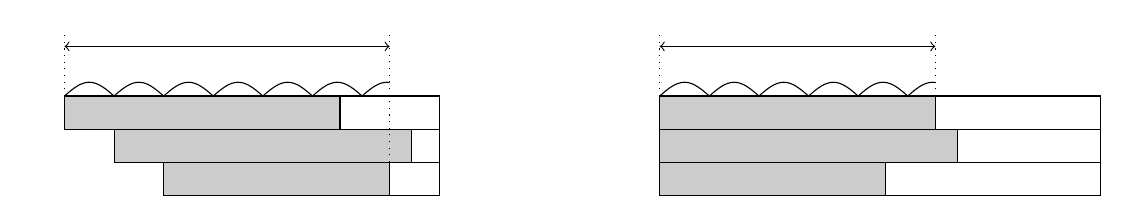
\begin{tikzpicture}[scale=0.7]



    \draw (3.2,0) rectangle (10, 0.6);

    \draw (2.7, .3) node[anchor=mid] {\footnotesize};
    
    \draw (4.1,-.6) rectangle (10, 0);
    \draw (3.6, -.3) node[anchor=mid] {\footnotesize};
    \draw (5,-1.2) rectangle (10, -0.6);
    \draw (4.5, -.9) node[anchor=mid] {\footnotesize};
    
    \filldraw[fill=black!20] (3.2,0) rectangle (8.2,0.6);
    \filldraw[fill=black!20] (4.1,-.6) rectangle (9.5,0);
    \filldraw[fill=black!20] (5,-1.2) rectangle (9.1,-0.6);

    \begin{scope}
        \clip (3.2,0) rectangle (9.1, 1);
        \foreach \x in {0, 0.9, ..., 10} {
          \draw (3.2+\x, .6) sin (3.2+\x+.45, .85) cos (3.2+\x+.9, .6);
        }
    \end{scope}
    
    
        \draw[<->] (3.2, 1.5) -- node[anchor=mid,above=-0.09]{\footnotesize } (9.1, 1.5);
         \draw[dotted] (3.2,0.6)--(3.2,1.7)   (9.1, -1.2)--(9.1, 1.7);
        \draw (3.65, 1.05) node {\footnotesize };

    \begin{scope}[xshift = 14 cm]
    \foreach \x in {0,1,2}{
        \draw (0,0-\x*0.6) rectangle (8,.6-\x*0.6);
        \draw (-.5, .3-\x*0.6) node[anchor=mid] {\footnotesize};
        }
        
        \filldraw[fill=black!20] (0,0) rectangle (5,0.6);
    \filldraw[fill=black!20] (0,-.6) rectangle (5.4,0);
    \filldraw[fill=black!20] (0,-1.2) rectangle (4.1,-0.6);

        \draw[<->] (0, 1.5) -- node[anchor=mid,above=-0.09]{\footnotesize } (5, 1.5);
        \draw (0.45, 1.05) node {\footnotesize };

        \draw[dotted] (0,0.6)--(0,1.7)   (5, .6)--(5, 1.7);

        \begin{scope}
            \clip (0,0) rectangle (5, 1);
            \foreach \x in {0, 0.9, ..., 11} {
                \draw (\x, .6) sin (\x+.45, .85) cos (\x+.9, .6);
            }
        \end{scope}

    \end{scope}

\end{tikzpicture}
\end{center}
 \caption{An illustration of notions used in \cref{lem:peralg}.
Shaded rectangles represent the common prefixes of  and .
In this case, .}\label{fig:perlcp}
\end{figure}

Although our applications use \cref{fct:lcp} for two different purposes,
the overall scheme is the same each time. Consequently, we group two application-specific queries
in a single algorithmic lemma; see \cref{fig:perlcp}.

\peralg*
\begin{proof}
There is nothing to do for .
For , \cref{fct:lce} lets us check if , that is, whether  matches a prefix of .
Moreover,  maximizes .

Henceforth, we shall assume . In this case, we retrieve an occurrence  of the string period  of  and apply \cref{fct:lce} to determine  and .
We also compute .

Let us observe that for , , so .
If , then .
Hence, by \cref{fct:lcp}, we have  for ,
 for  (if ),
and  for .

\ref{it:perpref}
We shall report  such that .
For , we have , so these indices are never reported.
If , we compute  using \cref{fct:lce} and this index may need to be reported.
For , we have  and , so we either report all these indices (if ) or none of them (otherwise).

\ref{it:permax}
If , we check whether  using \cref{fct:lce}.
If so, we report  as the only index maximizing  because  holds unless .
Otherwise, the maximum of  is~, attained for all  such that  (if ),
or~, attained for  (if ).
\end{proof}


\subsection{Prefix-Suffix Queries and Their Applications}\label{sec:BQ}
In this section, we show the solutions for \BQ, \PQ, and \PEQ using \IPM.

We start with \BQ. Assume that ; otherwise, there are no suffixes to be reported.
Let  be the prefix of  of length  and  be the suffix of  of length .
Suppose that a suffix  of  matches a prefix of . If , then  must start with a fragment matching~.
Moreover, if , then  is a suffix of , so this yields an occurrence of  in .
We find all such occurrences with a single \textsc{IPM Query} and then use \cref{lem:peralg} to find out which of them
can be extended to the sought suffixes  of .

\begin{figure}[ht]
\begin{center}
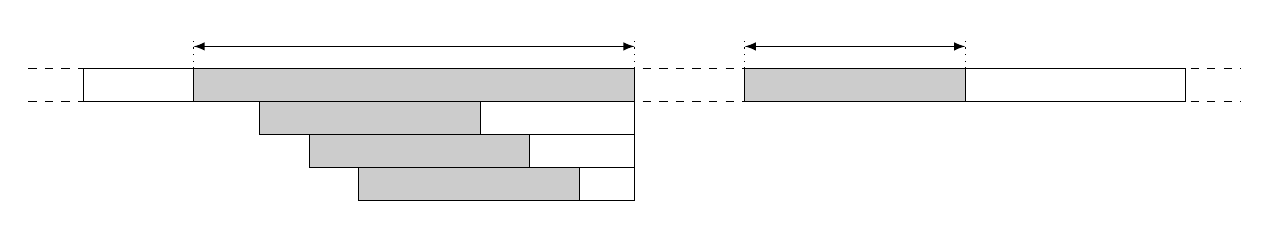
\begin{tikzpicture}[scale=0.7]

    \draw[dashed] (-1, 0)--(21, 0)  (-1, 0.6)--(21, 0.6);

    \draw (0,0) rectangle (10, 0.6);

    \draw (-.5, .3) node[anchor=mid] {\footnotesize};

    \filldraw[fill=black!20] (2,0) rectangle (10, .6);
    \draw (6, .3) node[anchor=mid] {\footnotesize};


    \draw[dotted] (2, 0.6) -- (2, 1.2) (10, 0.6) -- (10, 1.2);
        \draw[latex-latex] (2, 1) -- node[anchor=mid,above=-0.09]{\footnotesize } (10, 1);
    


    \foreach \i in {0,1,2} {
        \draw (3.2+0.9*\i, -0.6-0.6*\i) rectangle (10,-0.6*\i);
        \filldraw[fill=black!20] (3.2+0.9*\i, -0.6-0.6*\i) rectangle node[anchor=mid]{\footnotesize }(7.2+0.9*\i,-0.6*\i);
        \draw (2.7+0.9*\i, -0.3-0.6*\i) node[anchor=mid]{\footnotesize };
    }

    \begin{scope}[xshift = 12 cm]
        \draw (0,0) rectangle (8,.6);
        \draw (-.5, .3) node[anchor=mid] {\footnotesize};

        \filldraw[fill=black!20] (0,0) rectangle (4, .6);
        \draw (2, .3) node[anchor=mid] {\footnotesize};

        \draw[latex-latex] (0, 1) -- node[anchor=mid, above=-0.09]{\footnotesize } (4, 1);

        \draw[dotted] (0,0.6)--(0,1.2)  (4,0.6)--(4,1.2);

    \end{scope}

\end{tikzpicture}
\end{center}
 \caption{The notions used in the algorithms answering \BQ and \BLCP (for the latter, see \cref{sec:GSC}).}\label{fig:app-blcp}
\end{figure}

By \cref{fct:single}, the starting positions of the occurrences of  in  form a periodic progression in~.
Let  be the suffix of  starting with the th occurrence of ; see \cref{fig:app-blcp}.
We need to check which of the fragments  occur as prefixes of .
This is possible using \cref{lem:peralg}\ref{it:perpref}, which lets us find all indices  such that  is a prefix of .
The result is an integer interval of indices, which can be transformed into an arithmetic progression of lengths .
Consequently, the data structure of \cref{thm:ipm} (which already contains the component of \cref{prop:lce} for \LCEQ) can answer \BQ in  time.
Hence, we obtain the following results.

\thmappbq*


\thmapppq*

\begin{proof}
\PQ can be answered using \BQ for .
To compute all periods of , we use \BQ to find all borders of  of length within  for each .
The lengths of borders can be easily transformed to periods since  has period  if and only if it has a border of length .
\maybeqed \end{proof}


\thmrun*
\begin{proof}
  \PEQ can be answered using \BQ and \LCEQ in  and .
  Given a fragment , we use a \BQone to find the longest proper border of , provided that its length is at least .
  If no such border exists, we report that .
  Otherwise, the length of the longest border yields the period .
  In this case, 
  where  denotes the length of their longest common suffix of strings  and .
\maybeqed \end{proof}


\subsection{Cyclic Equivalence Queries}\label{sec:FC}

Recall that, for a non-empty string , we define a string .
First, we prove that the sought set 
indeed forms an arithmetic progression.

\begin{fact}\label{fct:FC}
  If , then  is an infinite arithmetic progression whose difference divides~.
\end{fact}
\begin{proof}
  Let us note that if , then  and thus also .
  Consequently,  consists of multiples of some integer .
  Due to , this integer  is a divisor of .

  Next, observe that if , then .
  Hence, if , then  is an infinite arithmetic progression whose difference divides .
\end{proof}

While answering \FC, we can assume that ;
we denote the common length of  and  by .
Our query algorithm is based on the following characterization of :

\begin{observation}\label{obs:rot}
Let  be strings of common length . For every ,
we have  if and only if  and .
\end{observation}


Below, we provide an algorithm that computes .
By \cref{obs:rot},  if and only if , so running this algorithm both for 
and  lets us retrieve .
This is sufficient to determine  because an \textsc{LCE Query} lets us easily check if , i.e., whether , and \cref{fct:FC} yields .

By \cref{obs:rot}, if ,
then the length- suffix of  matches a prefix of .
Since , all lengths  satisfying the latter condition form an arithmetic progression and can be retrieved with a single 
\textsc{Prefix-Suffix Query}. 
Moreover, \cref{obs:rot} yields .
Hence, it suffices to check for which indices  the suffix  of  matches a prefix of .
For this, we note that  is a periodic progression in :
for each , the string  matches a suffix of 
whose length is the difference of the arithmetic progression .
Hence, \cref{lem:peralg}\ref{it:perpref} lets us retrieve an integer interval
consisting of indices  such that , and this interval can be easily
transformed into an arithmetic progression of the corresponding values .
Consequently, the data structure of \cref{thm:ipm} (which already contains the component of \cref{prop:lce} for \LCEQ and which can answer \BQ in  time; cf.\ \cref{thm:app-bq})
can also answer \FC in  time.
 
\thmfc*

\subsection{Queries Related to Lempel--Ziv Compression}\label{sec:GSC}
\textsc{Substring Compression Queries} are internal queries asking for a compressed representation of a substring or the (exact or approximate) size of this representation.
This family of problems was introduced by Cormode and Muthukrishnan~\cite{DBLP:conf/soda/CormodeM05},
and some of their results were later improved by Keller et al.~\cite{DBLP:journals/tcs/KellerKFL14}.
\textsc{Substring Compression Queries} have a fairly direct motivation: 
Consider a server holding a long repetitive text  and clients asking for substrings of~ (e.g., chunks that should be displayed).
A limited capacity of the communication channel justifies compressing these substrings.

The aforementioned papers~\cite{DBLP:conf/soda/CormodeM05,DBLP:journals/tcs/KellerKFL14} apply the classic LZ77 compression scheme~\cite{DBLP:journals/tit/ZivL77}.
Among other problems, they consider internal queries for the LZ factorization of a given fragment 
and for the generalized LZ factorization of one fragment  in the context of another fragment .
The latter is defined as the part representing  in the LZ factorization of a string , 
where  is a special sentinel symbol not present in the text. 
A server can send such a generalized LZ factorization to a client who requests  and has previously received .

Thus, in this section, we consider variants of \LSC.
Let us first recall Lempel--Ziv LZ77 algorithm~\cite{DBLP:journals/tit/ZivL77} and range successor queries that will be used in our solution.

\paragraph{LZ77 Compression}
Consider a string . We say that a fragment  has a \emph{previous occurrence} (or is a \emph{previous fragment}) if  for some positions  and . The fragment  has a \emph{non-overlapping previous occurrence} (or is a \emph{non-overlapping previous fragment}) if additionally .

The Lempel--Ziv factorization  is a factorization  into fragments (called \emph{phrases}) such that 
each phrase  is the longest previous fragment starting at position ,
or a single letter if there is no such previous fragment.
The non-overlapping Lempel--Ziv factorization  is defined analogously, allowing for non-overlapping previous fragments only.
Both factorizations (and several closely related variants) are useful for compression
because a previous fragment can be represented using a reference to the previous occurrence (e.g., the positions of its endpoints).

Strings  are sometimes compressed with respect to a \emph{context string} (or \emph{dictionary string}) .
Essentially, there are two ways to define the factorization  of  with respect to .
In the \emph{relative LZ factorization}~\cite{DBLP:journals/tit/ZivM93,DBLP:conf/spire/KuruppuPZ10} , each phrase is the longest fragment of  which starts at the given position and occurs in  (or a single letter if there is no such fragment).
An alternative approach is to allow both substrings of  and previous fragments of  as phrases. This results in the \emph{generalized LZ factorization}, denoted ; see~\cite{DBLP:conf/soda/CormodeM05,DBLP:journals/tcs/KellerKFL14}.
Equivalently,   can be defined as the suffix of  corresponding to , where  is a special symbol that is present neither in  nor in .
The previous fragments in the non-overlapping generalized LZ factorization  must be non-overlapping.
\begin{example}
Let  and .
We have

\end{example}

\paragraph{Range Successor Queries}
We define the \emph{successor} of an integer  in a set  as
.
Successor queries on a range  of an array  are defined as follows.
\defdsproblem{\textsc{Range Successor Queries (Range Next Value Queries)}}{
  \textbf{Input}: An array  of  integers.\\
\textbf{Queries} Given a range  and an integer , compute  (and an index  such that , if any).}

The following three trade-offs describe the current state of the art for such queries.
\begin{proposition}\label{prp:range_successor_ub}
For any constant  and the functions , , and  specified below, there is a data structure of size 
  that answers range successor queries in  time and can be constructed in  time:
 \begin{enumerate}[label=(\alph*)]
   \item\label{it:succn} , ,
   and ~\cite{DBLP:conf/swat/NekrichN12,DBLP:conf/soda/BelazzouguiP16};
   \item\label{it:succloglog} , , and ~\cite{DBLP:journals/ipl/Zhou16,Gao2020};
   \item\label{it:succeps} , ,
   and ~\cite{DBLP:journals/tcs/CrochemoreIKRTW12}.
 \end{enumerate}
\end{proposition}


\paragraph{LZ Substring Compression Queries}
We consider the following types of queries.
\defdsproblem{\textsc{(Non-Overlapping) LZ Substring Compression Queries}}{
Given a fragment  of , compute the (non-overlapping) LZ factorization of , i.e.,  (, respectively).
}
\defdsproblem{\textsc{Relative LZ Substring Compression Queries}}{
Given two fragments  and  of , compute the relative LZ factorization of  with respect to , i.e., .
}

\defdsproblem{\textsc{Generalized (Non-Overlapping) LZ Substring Compression Queries}}{
Given two fragments  and  of , compute the generalized (non-overlapping) LZ factorization of  with respect to , i.e., 
(, respectively).
}

Our query algorithms heavily rely on the results of Keller et al.~\cite{DBLP:journals/tcs/KellerKFL14} for \LSC and \GSC. 
The main improvement is a more efficient solution for the following auxiliary problem:
\defdsproblem{\BLCPFull}{Given two fragments  and  of , find the longest prefix  of  which  occurs in .}
The other, easier auxiliary problem defined in~\cite{DBLP:journals/tcs/KellerKFL14} is used as a black box.
\defdsproblem{\ILCPFull}{Given a fragment  of  and an interval  of positions in , 
find the longest prefix  of  which occurs in   at some position within .}

The data structure for \ILCP uses range successor queries, so we state the complexity in an abstract form.
This convention gets propagated to further results in this section.

\begin{lemma}[Keller et al.~\cite{DBLP:journals/tcs/KellerKFL14}]\label{lem:app-ilcp}
For a text  of length , there exists a data structure of size  that answers \ILCP\ in  time.
The data structure can be constructed in  time.
\end{lemma}

As observed in~\cite{DBLP:journals/tcs/KellerKFL14}, the decision version of \IPM easily reduces to \ILCP. For 
and , it suffices to check if the longest prefix of  occurring at some position in  of  is  itself.\begin{corollary}[Keller et al.~\cite{DBLP:journals/tcs/KellerKFL14}]\label{lem:any}
For a text  of length , there exists a data structure of size  that, given fragments  of , can decide in  time whether  occurs in .
The data structure can be constructed in  time.
\end{corollary}

We proceed with our solution for \BLCP.
Let  and .
First, we search for the largest  such that the prefix of  of length~ (i.e., ) occurs in .
We use a variant of the binary search involving exponential search (also called galloping search),
which requires  steps, where  is the optimal value of .
At each step, for a fixed  we need to decide if  occurs in .
This can be done in  time using \cref{lem:any}.
At this point, we have an integer  such that the optimal prefix  has length .
The running time is  so far.

Let  be the prefix obtained from an \textsc{Interval Longest Common Prefix Query} for  and .
We have  and thus the occurrence of  starting in  lies within .
Consequently, ; moreover, if  occurs at a position within ,
then .

The other possibility is that  only occurs near the end of , i.e., within the suffix of  of length , which we denote as .
We use a similar approach as for \BQ with  to detect  in this case.
We define  as the prefix of  of length .
An occurrence of  must start with an occurrence of , so we find all occurrences of  in .
If there are no such occurrences, we conclude that .

Otherwise, we define  as the suffix of  starting with the th occurrence of ; see~\cref{fig:app-blcp}.
Next, we apply \cref{lem:peralg}\ref{it:permax} to compute . By the discussion above,
this must be the length of the longest prefix of  which occurs in .
We compare its length to  and choose the final answer  as the longer of the two candidates.

Thus, the data structure for \IPM, accompanied by the components of \cref{lem:app-ilcp,lem:any,prop:lce},
yields the following result:

\thmblcp*

Finally, we generalize the approach of~\cite{DBLP:journals/tcs/KellerKFL14} to support multiple types of \LSC using \cref{thm:blcp} to improve the running time.


\begin{theorem}\label{thm:lsc}
For every text  of length , there is a data structure of size 
that answers:
\begin{enumerate}[label=(\alph*)]
  \item \textsc{Non-Overlapping} \LSC,
  \item \textsc{Relative} \LSC,
  \item \GSC, and
    \item \textsc{Generalized Non-Overlapping} \LSC,
\end{enumerate}
each in  time,
where  is the number of phrases reported.
The data structure can be constructed in  time.
\end{theorem}
\begin{proof}
Let  and suppose that we have already factorized ,
i.e., the next phrase needs to be a prefix of .
Depending on the factorization type, it is chosen among the longest prefix of  that is a previous fragment of  (i.e., has an occurrence starting within ), the longest prefix of  that is a non-overlapping previous fragment of  (i.e., occurs in ),
or the longest prefix of  that occurs in .
The first case reduces to an \textsc{Interval Longest Common Prefix Query}, while the latter two---to \BLCP.
For each factorization type, we compute the relevant candidates and choose the longest one as the phrase;
if there are no valid candidates, the next phrase is a single letter, i.e., .

Thus, regardless of the factorization type, we report each phrase  of the factorization 
in  time. 
This way, the total running time is , which is   due to Jensen's equality applied to the concave  function.
\maybeqed \end{proof}

Let us note that in the case of ordinary \LSC the approach presented in \cref{thm:lsc} would result in  query time
because only \ILCP would be used; this is exactly the algorithm for \LSC provided in~\cite{DBLP:journals/tcs/KellerKFL14}.

Hence, despite our improvements, there is still an overhead for using variants of the LZ factorization other than the standard one.
Nevertheless, the overhead disappears if we use the state-of-the-art -size data structure for range successor queries. This is because the  time complexity lets us hide  factors
by choosing a slightly greater .
Formally, \cref{thm:lsc,prp:range_successor_ub} yield the following result:
\begin{corollary}\label{cor:app-blcp}
For every text  of length  over an alphabet  and constant , there is a data structure of size 
that answers \BLCP\ in  time
and \LSC (for all five factorization types defined above) in  time per phrase reported.
Moreover, the data structure can be constructed in  time.
\end{corollary}


\section*{Acknowledgement}
The authors wish to thank Dominik Kempa for helpful discussions regarding synchronizing sets
and Moshe Lewenstein for a suggestion to work on the Generalized Substring Compression problem.
Jakub Radoszewski was supported by the Polish National Science Center, grant no.\ 2022/46/E/ST6/00463.

\bibliographystyle{alphaurl}
\bibliography{ipm}

\appendix

\section{Proof of \cref{lem:maxcut}}\label{app:AMDC}

\AMDC*
\begin{proof}
First, we preprocess  so that each  stores both incoming and outgoing arcs.
For , we denote  to be the set of arcs leading from  to ;
recall that the goal is to make sure that .
Given  and , define 
and .

We maintain a partition  into three disjoint classes.
Initially,  and, as long as , we pick an arbitrary vertex 
and move  to  or , depending on whether 
or not.
This decision can be implemented in  time, which yields a total running time of .

As for correctness, we shall prove that 
cannot decrease throughout the algorithm.
Consider the effect of moving  from  to  on the four terms of~ (recall that there are no self-loops ):
\begin{itemize}
  \item  increases by ;
  \item  increases by  and decreases by ;
  \item  decreases by ;
  \item  decreases by  and decreases by .
\end{itemize}
Overall,  increases by 
  
and this quantity is non-negative when the algorithm decides to move  to . 

Similarly, if  is moved from  to , then  does not decrease.
Upon the end of the algorithm, we have  due to ,
whereas, initially,  due to . 
Since  is non-decreasing, we conclude that  holds as claimed. 
\end{proof}

\end{document}
